
\documentclass[
  reprint,            % journal-like 2-column
  amsmath,amssymb,    % math packages
  aps,pre,              % APS + Physical Review E style    
  superscriptaddress        
]{revtex4-2}

% ---- Core packages APS samples rely on ----
\usepackage{graphicx} % \inputgraphics
\usepackage{dcolumn}  % decimal-aligned tables
\usepackage{bm}       % bold math
\usepackage[T1]{fontenc}
\usepackage[utf8]{inputenc}

% Hyperlinks (APS allows it; keep unobtrusive)
\usepackage[colorlinks=true, allcolors=blue]{hyperref}


% PACKAGES FOR LANGUAGE AND FONT
\usepackage{verbatim} % For code blocks

% PACKAGES FOR ALGORITHMS (PSEUDO-CODE)
\usepackage{etoolbox} 
\usepackage{algorithm}

% PACKAGES FOR IMAGES
\usepackage{tikz} % A package for high-quality hand-made figures.
\usetikzlibrary{}
% \usepackage{float}
\usepackage[percent]{overpic} % For adding annotations to figures
% \usepackage{graphbox} 

% FOR TABLES
\usepackage{array}     % enables m{...}, >{...}, \arraybackslash, etc.
\usepackage{booktabs}  % enables \toprule \midrule \bottomrule

% STANDARD MATH PACKAGES
\usepackage{mathtools}
\usepackage{cases}
\usepackage{xfrac}

% OTHER PACKAGES
\usepackage{lipsum} % DUMMY PACKAGE

% Graphics search paths
\graphicspath{{Images/}}

% Miscellaneous operators
\DeclareMathOperator{\arctanh}{arctanh}

\newcommand{\bea}{\begin{eqnarray}} % Shortcut for equation arrays
\newcommand{\eea}{\end{eqnarray}}
\newcommand{\e}[1]{\times 10^{#1}}  % Powers of 10 notation
\def\norm#1{\|#1\|} %Norm

% Commonly used symbols
\renewcommand{\a}{\alpha}
\renewcommand{\b}{\beta}
\renewcommand{\k}{\kappa}
\newcommand{\w}{\omega}
\newcommand{\wB}{\omega_B}
\newcommand{\wZ}{\omega_0}
\newcommand{\wz}{\omega_z}
\newcommand{\wpm}{\omega_\pm}
\newcommand{\neff}{n_{eff}}
\newcommand{\dn}{\delta n}
\newcommand{\dnbar}{\overline{\delta n}_{eff}}
\newcommand{\dt}{\delta \tau}

\newcommand{\Skenderas}{Sk\"{e}nderas}

\pdfpageattr{/Rotate 0}

% =======================
% Document
% =======================
\begin{document}

\preprint{APS/123-QED} % optional

\title{Modelling and Analysis of Semiconductor Lasers Under Fiber Bragg Grating Feedback}

\author{J. Steele}
\email{jste924@aucklanduni.ac.nz}
\affiliation{Dodd--Walls Centre for Photonic and Quantum Technologies, New Zealand}
\affiliation{Department of Mathematics, University of Auckland, New Zealand}

\author{B. Krauskopf}
\affiliation{Dodd--Walls Centre for Photonic and Quantum Technologies, New Zealand}
\affiliation{Department of Mathematics, University of Auckland, New Zealand}

\author{N. Broderick}
\affiliation{Dodd--Walls Centre for Photonic and Quantum Technologies, New Zealand}
\affiliation{Department of Physics, University of Auckland, New Zealand}


\date{\today}

% ---- Abstract kept modular: put the whole environment in Sections/Abstract.tex ----

% !TeX root = ../main.tex

\begin{abstract}
Semiconductor lasers are compact, efficient light sources widely used in optical communications, and their sensitivity to external feedback makes them rich systems for studying nonlinear dynamics. 
The Lang-Kobayashi (LK) equations are the standard tool for modelling lasers subject to external feedback from a regular mirror. 
A key reflective component in optical systems is the fiber Bragg grating (FBG)—a periodic optical fiber refractive index variation—leveraged for its precise spectral control and all-fiber compatibility. 
When the external feedback comes from an FBG, present modelling requires a computationally expensive convolution term, which provides limited analytical insight into the system's behaviour. 
We present a novel modelling approach that approximates FBG feedback by a sum of discrete delay terms. Critically, this avoids the need for numerical convolution while preserving the essential physics. 
This enables detailed analysis of the laser’s mode structure, stability regimes, and bifurcation structure in the spirit of that for the `classic' LK equations. 
In this way, our work provides a foundation for deeper theoretical study of semiconductor lasers subject to technologically relevant types of FBG feedback, bridging the gap between numerical simulation and analytical understanding.
\end{abstract}


%\keywords{Suggested keywords}%Use showkeys class option if keyword
                              %display desired

\maketitle

% =======================
% Main text (modular)
% =======================
% Use \input so each section gets its own .aux (these will land in build/Sections/ with your latexmkrc)
% File names below are examples; create the matching files in Sections/ with no spaces in names.
% !TeX root = ../main.tex
\section{Introduction}
\label{sec:introduction}
%
Semiconductor lasers are fundamental components in modern photonic technologies.
Most importantly, their emission wavelengths align with those used in optical communication networks, making them valuable light sources.
In addition, they are orders of magnitude smaller than typical helium–neon lasers, with coherence lengths of only a few millimetres compared to many metres, which enables widespread practical applications \cite{heiskanen2018photobiomodulation}.
Semiconductor lasers are not only smaller than conventional gas lasers, but also exhibit much higher output coupling, with approximately 70\% of the light intensity escaping them compared to 1-5\% for gas lasers \cite{vantartwijk1995semiconductor}.
However, this openness makes semiconductor lasers more susceptible to external disturbances, leading to a strong response to incident signals.
Although undesirable in some practical applications, this sensitivity has made semiconductor lasers a central platform for investigating nonlinear dynamics induced by external optical feedback.
The influence of external light on laser operation has been extensively investigated since the 1970s, with particular focus on conventional optical feedback (COF) (typically achieved by reflecting output laser light back into the laser cavity using a mirror) as well as on optical injection of laser light from another laser \cite{weiss1991dynamics}.
Feedback and injection mechanisms have important practical implications: for example, the former arises in the operation of CD players, while the latter is central to laser amplification systems.
Beyond their direct historical significance, semiconductor lasers with feedback underpin key technologies in modern photonics.
Feedback control is exploited to stabilize frequency and linewidth in coherent optical communication \cite{tkach2003regimes}, to enhance sensitivity in precision sensing and metrology, and to enable secure chaos-based encryption schemes \cite{uchida2008fast}.
At the same time, semiconductor lasers with feedback provide a prototypical and experimentally accessible example of delay differential equations (DDEs), serving as a platform to study nonlinear dynamics with relevance extending to control theory \cite{stepan1989retarded}, electronics, and biological systems \cite{mackey1977oscillation}.
%
%
\subsection*{Lang-Kobayashi equations}
A major breakthrough in understanding the dynamics of semiconductor lasers with external feedback came in 1980 with the seminal work of Lang and Kobayashi, who introduced what are now known as the Lang–Kobayashi (LK) rate equations.
These equations provide a description of the coupled carrier and optical field dynamics of a semiconductor laser subject to COF from a distant mirror \cite{lang1980external}.
These equations describe the coupled dynamics of the complex electric field $E = E_x + iE_y$ and the carrier inversion $N$ in a semiconductor laser subject to COF from a distant mirror \cite{lang1980external}.
A nondimensionalized form of these equations, highlighting the key parameters governing the system dynamics, is given by \cite{heil2003delay}
%
\begin{equation}
\label{eq:LK}
    \begin{aligned}
        \frac{d E}{d t} & =(1+i \a) N(t) E(t)+\eta F(t) \\
        T \frac{d N}{d t} & =P-N(t)-(1+2 N(t))|E(t)|^2
    \end{aligned}
\end{equation}
%
where the feedback term is given by $F(t) = e^{-i \w_0 \tau} E(t-\tau)$.
These key parameters can be separated into intrinsic laser parameters and external cavity (EC) parameters.
The laser, emitting at a single frequency $\w_0$, is characterised by the pump current $P$, the linewidth enhancement factor $\a$, and the ratio of photon and electron decay times $T = \tau_e/\tau_p$.
The external cavity (EC), which in this context is implemented as an optical fibre with refractive index $n_{eff}$, is characterised by the round-trip delay time $\tau = 2L_\text{EC}/n_{eff} c$, the feedback power level (defined as the ratio of power reflected from the external mirror to that from the diode mirror) $\eta$, and the feedback phase $C_p = \w_0 \tau$, corresponding to the number of optical wavelengths in the EC.
It is noted that these equations are formulated with reference to the centre frequency of the laser, with $\wZ = 0$ at the operating frequency, which implies $C_p = 0$ in the first instance.
The application of these equations requires a single-mode laser subject to weak feedback (up to a few percent of the emitted light) from a long EC, typically ranging from centimetres to metres in length.
These assumptions impose several important limitations on the LK model, which can be grouped into restrictions on the laser operating frequency, the cavity, and the feedback strength.
As the LK equations assume single-mode operation, they do not capture mode competition or spectral dynamics; for approaches to the analysis of multimode lasers, see \cite{yacomotti2004dynamics} and references therein.
A long EC justifies treating the feedback phase $C_p$ as an independent parameter from the delay $\tau$, since a $2\pi$ phase shift corresponds to only a half-wavelength change (about one micron) in the cavity length, which is negligible at these scales \cite{green2006mode}.
In practice, varying $C_p$ over a full $2\pi$ is achieved by shifting the mirror position using a piezoelectric transducer \cite{heil2003delay} for example, or by changing thermal properties of the cavity itself, introducing a slight variation to the fibre's refractive index and thus effective cavity length \cite{skenderas2021feedback}.
The weak-feedback condition further ensures that multiple EC reflections between the laser facet and the external mirror can be neglected; if this condition is not satisfied, the feedback $F(t)$ takes a more complex form \cite{vantartwijk1995semiconductor}.
%
\begin{equation}
\label{eq:multiple_EC}
    F(t) = \frac{R_2^{\;2} - 1}{R_2^{\;2}} \sum_{n=1}^\infty (-R_2 R)^n e^{-i n C_p} E(t-n \tau)
\end{equation}
%
where $R$ is the reflectivity of the external mirror and $R_2$ is the reflectivity of the laser facet.
%
\par
%
The LK equations successfully capture the rich dynamical behaviours of semiconductor lasers under weak external feedback, including steady-state, periodic, quasi-periodic, and chaotic emission, as well as complex behaviours such as regular pulse packages (RPPs), coherence collapse (CC), and low-frequency fluctuations (LFFs) \cite{heil1998coexistence}.
The delay $E(t-\tau)$ present in the feedback term $F(t)$ makes the LK equations DDEs with phase space in the infinite-dimensional Banach space $C([-\tau,0],\mathbb{C}\times\mathbb{R})$, consisting of continuous functions that describe the past history of the optical field.
Due to the rotational symmetry of the complex field $E$, the effective phase space is this function space modulo the action of $\mathrm{S}^1$.
This memory effect, arising from time-delayed optical feedback whereby the system evolves according to both its current and past states, is absent in injected semiconductor laser systems, where dynamics are instead dominated by phase-locking and frequency pulling \cite{wieczorek1999unifying,wieczorek2005dynamical}.
The success of the LK equations stems from their role as a minimal yet sufficient model: a coupled nonlinear DDE system that reproduces experimentally observed behaviours while remaining amenable to rigorous analysis.
In this framework, equilibria can be analysed in detail, yielding a clear picture of local dynamics \cite{rottschafer2007ecm}.
Moreover, numerical continuation tools for DDEs, such as \texttt{DDE-Biftool}, enable systematic tracking of equilibria and periodic orbits, as well as the detection of secondary bifurcations that organise the global dynamics \cite{sieber2014dde, krauskopf2004dynamics}.
%
\par
%
A central insight of the LK model is the structure of its steady states, known as external cavity modes (ECMs).
The ECMs form an ellipse in frequency space centred at the free-running laser frequency, with the maximum gain mode (MGM) located on the outer boundary, farthest from the centre frequency.
The number of ECMs and the frequency interval they occupy increase with feedback strength and EC length.
ECMs are typically created in saddle-node pairs as parameters vary, and their stability changes through Hopf bifurcations \cite{heil2003delay, rottschafer2007ecm}.
The set of ECMs provides the backbone of the LK dynamics: it organises transients and families of periodic and quasi-periodic orbits that arise from Hopf and subsequent bifurcations.
In regimes such as LFFs and CC, trajectories spend long intervals near weakly stable ECMs before departing along unstable manifolds of neighbouring saddle ECMs, producing intensity dropouts.
The prevalence and severity of these behaviours increase with the size of the ECM ellipse \cite{heil2003delay, krauskopf2004dynamics}.
Thus, understanding the geometry, multiplicity, and stability of ECMs is essential for explaining observed dynamical regimes and for devising control strategies.
This perspective naturally motivates efforts to reduce or confine the set of accessible ECMs, thereby enhancing stability under stronger feedback by limiting the number of available steady-states.
A crucial step in this direction is understanding how different forms of feedback, beyond COF, can suppress or restructure the ECM ellipse, providing new routes to controlled laser dynamics.
%
%
\subsection*{Phase-conjugate feedback}
\label{subsec:PCF}

In a single-mode semiconductor laser with phase-conjugate feedback (PCF), the phase-conjugating mirror (PCM) returns a wavefront-inverted replica of the emitted light.
This self-aligning feedback, typically realised through degenerate four-wave mixing in vapours or semiconductors, or by gratings and optical crystals, compensates distortions in the EC.
By reversing wavefront errors on each round trip, phase conjugation stabilises both beam quality and frequency, motivating its application in semiconductor laser control.
Owing to these potential stabilisation features, PCF was among the earliest feedback configurations investigated beyond COF \cite{krauskopf1998semiconductor, green2004bifurcation}.
In the standard LK rate-equation framework \eqref{eq:LK}, PCF is represented by a delayed conjugated field term, $F(t) = e^{-i \phi_\text{PCM}} E^*(t-\tau)$, which yields a DDE system with discrete $\mathbb{Z}_2$ symmetry $E \rightarrow -E$ \cite{krauskopf2002routes}.
This symmetry leads to qualitative differences in the mode structure.
Whereas COF produces a continuous ellipse of ECMs organised by the feedback phase, PCF gives rise instead to isolated branches of ECMs whose frequencies are locked near integer multiples of the cavity frequency \cite{erneux2003external}.
Within the locking range, the PCF laser is both frequency- and phase-locked to the pump, and unlike COF, phase locking does not depend on the feedback phase.
Overall, the resulting linewidth is ultranarrow and robust against added noise \cite{green2002global}.
Because the feedback term retains the same discrete DDE form of the LK equations, PCF remains analytically tractable and compatible with numerical bifurcation tools such as continuation, which has enabled detailed exploration of its mode structure and stability.
%
\subsection*{Filtered optical feedback}
\label{subsec:FOF}
%
The most direct method of controlling the ECMs in a semiconductor laser is to filter the light fed back into the cavity, a scheme known as filtered optical feedback (FOF).
By modifying the spectrum of the reinjected light, FOF reshapes the set of accessible ECMs.
Several practical implementations of FOF have been investigated.One approach is the insertion of a Fabry–Pérot resonator within the feedback loop \cite{detienne1997semiconductor}.
More commonly, the external mirror is replaced by a frequency-selective surface, such as a grating \cite{dahmani1987frequency, harvey1991external, jin1996single}, or by a phase-conjugating surface, for example a Kerr-type nonlinear medium, which in this context acts primarily as a spectral filter \cite{agrawal1984line}.
As expected, all of these implementations lead to significant linewidth narrowing, resulting in more stable operation around the filter’s free-running frequency.
This makes FOF a practical approach for stabilising single-mode operation and narrowing emission spectra in photonic applications.
%
\par
%
Mathematical analysis of FOF poses additional challenges not encountered with COF or PCF.
In this case, the spectral components of the electric field must be included explicitly, since their reflection is governed by the frequency response of the chosen filter, denoted $\rho(\w)$.
Therefore, the feedback term $F(t)$ must be replaced by a more general expression that accounts for this frequency selectivity.
For a given reflection response, $F(t)$ can be obtained by decomposing the field into its Fourier components, applying the filter’s reflection spectrum $\rho(\w)$, and then taking the inverse Fourier transform \cite{yousefi1999dynamical}.
Mathematically, this amounts to
%
\begin{equation}
    \begin{aligned}
    \label{eq:FOF}
         F(t) &=  \mathcal{F}^{-1}\big[ \mathcal{F}[E(t)](\w) \times \rho(\w) \big](t-\tau)\\
              &= \frac{1}{2\pi} \int_{-\infty}^{\infty} \rho(\w) \int_{-\infty}^{\infty} E(t') e^{-i \w t'} dt' e^{i \w (t-\tau)} d\w.
    \end{aligned}
\end{equation}
%
This expression highlights that the feedback is no longer a simple delayed replica of the field, but a spectrally filtered version shaped by $\rho(\w)$.
Unlike COF and PCF, FOF directly reshapes the spectral window of accessible ECMs.
Note that \eqref{eq:FOF} again assumes a single reflection is sufficient to describe the external feedback signal $\eta F(t)$.
The distributed nature of the feedback expressed in \eqref{eq:FOF} makes the system difficult to treat analytically and computationally demanding to simulate.
The modified LK equations take the form of integro-differential equations that are not amenable to standard bifurcation analysis tools, such as fixed-point calculation and stability analysis, which obscures even basic insights into the influence of filtering on the system.
Furthermore, numerical methods such as direct time-series integration of \eqref{eq:LK} become significantly more computationally demanding, since \eqref{eq:FOF} must be re-integrated at every time step, rather than simply retrieving the stored value $E(t-\tau)$ as in the standard LK equations.
%
\par
%
A key insight was provided in 1999 by Yousefi and Lenstra \cite{yousefi1999dynamical}, who assumed that filtering yields a frequency-dependent reflection spectrum $\rho(\w)$ represented as a sum of Lorentzians.
By considering a single Lorentzian, which can adequately describe certain external feedback mechanisms \cite{dahmani1987frequency,detienne1997semiconductor}, they showed that the integro-differential equations in this scheme can be reduced to a system of DDEs.
Specifically, the first two equations remain identical to the standard LK system, while the effect of filtering is incorporated by coupling an additional equation for $F(t)$.
%
\begin{equation}
\label{eq:FOF_LK}
    \frac{d F}{d t} = \Lambda E(t-\tau) e^{-i C_p}+(i \Delta-\Lambda) F(t)
\end{equation}
%
Here, $\Lambda$ is the full width at half maximum (FWHM) of the Lorentzian filter, which sets its spectral width, and $\Delta$ is the detuning of the filter from the laser’s free-running frequency.
Since coupling \eqref{eq:FOF_LK} to the standard LK equations \eqref{eq:LK} again yields a system of DDEs, the model remains amenable to the same analytical and numerical methods as the original LK system.
They demonstrated that, as expected, the system generally admits fewer external filtered modes (EFMs) (that is, the ECM modse when employing FOF) than COF and that, overall, filtering leads to more stable dynamics.
Alongside the reduction in the number of accessible ECMs, the MGM tends to lie closer to the filter frequency (though not exactly at it) rather than at the edge of the fixed-point ellipse as in COF.
Overall, the formulation of these equations as coupled DDEs allows for detailed investigation through continuation and stability analysis of the stationary states, providing deeper insight into the influence of FOF on semiconductor lasers 
\cite{erzgraber2006frequency, erzgraber2007bifurcation, erzgraber2007dynamics, fischer2000experimental, fischer2004experimental, green2006mode, 
hek2007semiconductor, erzgraber2007feedback, fischer2004filtered, yousefi2001global, yousefi2002simulations, yousefi2003nonlinear}.
%
\par
%
It has been shown that the EFM can undergo a fundamental topological change, splitting into two disconnected components when the filter is sufficiently detuned.
This breakup is organised by codimension-two and codimension-three bifurcations, which act as organising centres for the stability boundaries of EFMs in the filter–detuning parameter plane.
Continuation methods allow these bifurcations, along with the folds and Hopf curves that emanate from them, to be systematically tracked, providing a precise map of where mode break-up, relaxation oscillations, and frequency instabilities arise.
The result is a comprehensive picture in which analytic steady-state solutions and numerical continuation of equilibria and periodic orbits combine to reveal not only the number and arrangement of EFMs, but also the mechanisms by which their stability changes.
In this way, FOF has become one of the most thoroughly understood feedback configurations, demonstrating the level of insight that becomes possible when analytic tractability and continuation-based analysis can be brought together.
%
%
\subsection*{Fibre Bragg grating feedback}
\label{subsec:FBG_LK}
%
\subsubsection*{Fibre Bragg gratings}
\label{subsubsec:FBG}
%
One reflective frequency-dependent component that has been the focus of extensive research in recent decades is the fibre Bragg grating (FBG).
FBGs offer several advantages over other fibre-optic technologies.
These include all-fibre design, low insertion loss, high return loss, potential for lower cost, and, most notably, exceptional flexibility in tailoring spectral characteristics.
With current manufacturing techniques, gratings can be fabricated with nearly arbitrary spectral responses and normalised bandwidths ranging from $10^{-4}$ to $0.1$ \cite{erdogan1997fibre}.
The FBG is therefore a natural reflective element for implementing FOF.
%
\begin{figure}
    \centering 
    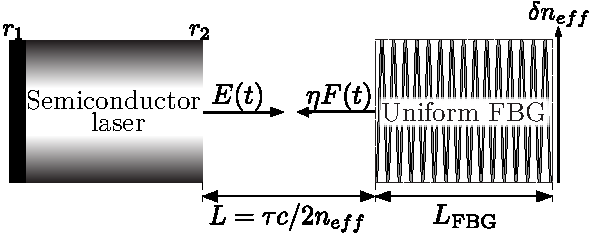
\includegraphics[width=\linewidth]{Images/FBG_setup_dneff_only_1col.pdf}
    \caption{Sketch of an optical fibre with an FBG written along its length.}
    \label{fig:FBG_setup}
\end{figure}
%
\par
%
An FBG is defined as a periodic modulation $\delta n_{eff}(z)$ of the refractive index with period $\Lambda$ along an optical fibre of length $L_\text{FBG}$.
The number of gratings in an FBG is therefore $N = L_\text{FBG}/\Lambda$.
The most general form of this periodic modulation is
%
\begin{equation}
\label{eq:dneff}
    \delta n_{eff}(z) = \dnbar(z) \left[ 1 + v \cos{\left( \frac{2 \pi}{\Lambda} z + \phi(z) \right)} \right].
\end{equation}
%
Here, $\dnbar(z)$ describes the envelope of the periodic modulation along $L_\text{FBG}$; for example, $\dnbar(z) \sim e^{-z^2}$ yields a Gaussian refractive index profile.
In addition to the envelope, $v$ denotes the fringe visibility of the index modulation, and $\phi(z)$ allows variation of the grating period along the fibre, enabling different frequencies to be reflected at different positions.
This flexibility allows tailoring of the spectral response through modulation depth and phase, directly influencing the accessible ECM structure.
%
\par
%
Light propagating in the fibre and interacting with the FBG undergoes diffraction when its wavelength is close to the design wavelength, $\lambda_D = 2 n_{eff} \Lambda$.
It is typically assumed that the light undergoes only first-order diffraction, which dominates in FBGs, so that a single propagating mode need be considered.
In this case, using coupled-mode theory and the synchronous approximation, one can derive coupled first-order differential equations describing the interaction between the forward- and backward-propagating waves, $R(z)$ and $S(z)$, respectively.
%
\begin{equation}
\label{eq:wave_eqs}
    \begin{aligned}
        \frac{dR}{dz} &= i \hat{\sigma} R(z) + i \k S(z) \\
        -\frac{dS}{dz} &= i \hat{\sigma} S(z) + i \k R(z)
    \end{aligned}
\end{equation}
%
with $R(z) = A(z) \exp{ \left( -i \left( \phi/2 -\delta z \right) \right) }, \; S(z) = B(z) \exp{ \left( -i \left( \phi/2 + \delta z \right) \right) }$.
For further details, see \cite{erdogan1997fibre} and references therein.
The parameters $\delta$, the wavevector mismatch, $\kappa$, the alternating-current (AC) coupling coefficient, and $\hat{\sigma}$, the direct-current (DC) self-coupling coefficient, are given by
%
\begin{align}
    \label{eq:delta}
    \delta &= 2 \pi \neff \left( \frac{1}{\lambda} - \frac{1}{\lambda_D} \right) \\
    \label{eq:kappa}
    \k &= \frac{\pi}{\lambda} v \dnbar(z)\\
    \label{eq:sigma}
    \hat{\sigma} &= \frac{2\k}{v} + \delta -\frac{1}{2}\frac{d\phi}{dz}.
\end{align}
%
Since $\k$ and $\hat{\sigma}$ may depend on $z$, \eqref{eq:wave_eqs} cannot in general be solved analytically, but they can be readily solved numerically once $\Lambda$, $n_{eff}$, $\dnbar(z)$, $\phi(z)$, and $L_\text{FBG}$ are specified.
%
\par
%
At this point, all the necessary ingredients are in place to calculate the key characteristic of an FBG, its reflection spectrum $\rho(\w)$.
Physically, the primary interest lies in the reflection spectrum of light reflected at the front FBG interface, assuming no reflection from the back interface.
Therefore, \eqref{eq:wave_eqs} is typically solved by setting $z = 0$ at the midpoint of the FBG, imposing boundary conditions $R(-L_\text{FBG}/2) = 1$ and $S(L_\text{FBG}/2) = 0$, and integrating backwards from $L_\text{FBG}/2$ to $-L_\text{FBG}/2$
The amplitude reflection coefficient is then given by
%
\begin{equation}
\label{eq:rho}
    \rho_\text{FBG} = \frac{S(-L_\text{FBG}/2)}{R(-L_\text{FBG}/2)}
\end{equation}
%
which defines the reflection spectrum $\rho(\w)$.
Although \eqref{eq:wave_eqs} must generally be solved numerically and closed-form expressions for $\rho(\w)$ are rarely available, certain standard grating designs such as uniform or raised-cosine-apodised gratings admit analytic solutions and provide valuable insight into the typical properties of FBG reflection spectra.
Among the different grating profiles, the simplest and most widely studied is the uniform grating.
%
%
\subsubsection*{Uniform FBG reflection spectra}
\label{subsubsec:FBG_feedback}
%
The uniform FBG is the canonical case, characterised by a constant grating period and uniform modulation depth.
Beyond being analytically tractable, it is also widely fabricated, providing a baseline for more advanced apodised or chirped gratings and a useful reference for understanding how FBG feedback influences ECM control.
For uniform gratings, the grating chirp satisfies $\sfrac{d\phi}{dz} = 0$ and the apodisation $\dnbar = \text{const.}$, so that the grating index variation given by \eqref{eq:dneff} reduces to a sine wave, as shown in Figure~\ref{fig:FBG_setup}.
Therefore, $\k$ and $\hat{\sigma}$ are constant in $z$, which allows the reflection spectrum $\rho(\w)$ to be obtained analytically by solving \eqref{eq:wave_eqs} and then evaluating \eqref{eq:rho}.
%
\begin{equation}
\label{eq:uniform_rho}
    \rho = \frac{-\k \sinh\left( L_\text{FBG}\right)}{\hat{\sigma} \sinh\left(\gamma L_\text{FBG}\right) + i\gamma \cosh\left(\gamma L_\text{FBG}\right)}
\end{equation}
%
where $\gamma = \sqrt{\k^2 - \hat{\sigma}^2}$ determines whether the field decays or oscillates within the grating.
Several key features of the reflection spectrum $\rho(\w)$ are most clearly visualised by plotting it as a function of normalised frequency detuning while varying $\kappa L_\text{FBG}$ for a fixed $N$ \cite{erdogan1997fibre}.
%
\begin{equation*}
    \frac{\w - \w_\text{max}}{\w_\text{max}} = \frac{\hat{\sigma} L_\text{FBG}  }{\pi N}
\end{equation*}
%
Figure~\ref{fig:uniform_spectra_varykL} shows representative amplitude reflectivity and group delay spectra for three uniform gratings, plotted against normalised frequency detuning.
The gratings are centred at the common laser wavelength of 1550 nm, with $\kappa L_\text{FBG} \in {0.5, 2, 5}$ and a fixed $N = 5000$, chosen to illustrate weak, moderate, and strong coupling regimes.
Increasing $N$ (and thus $L_\text{FBG}$) results in a narrower reflection bandwidth, whereas decreasing $N$ (and thus $L_\text{FBG}$) produces a broader one, provided that $\kappa L_\text{FBG}$ remains constant.
The reflection spectrum consists of a main lobe and a series of side lobes, separated by reflection zeros that are symmetrically spaced in wavelength on either side of the main lobe.
For gratings with low $\kappa L_\text{FBG}$, such as 0.5, the main lobe has a bandwidth, defined as the interval between its reflection zeros, that is twice the width of the side lobes \cite{erdogan1997fibre}.
Evidently, increasing $\kappa L_\text{FBG}$ increases the grating's maximum reflectivity and also broadens the main-lobe bandwidth while narrowing that of the side lobes.
Additionally, the time delay is approximately constant for low reflectivities but becomes increasingly distorted as $\kappa L_\text{FBG}$ increases.
Away from the main lobes, the time delays across all three cases are approximately the same, due to keeping the number of grating periods $N$ constant.
%
\begin{figure}[!t]
    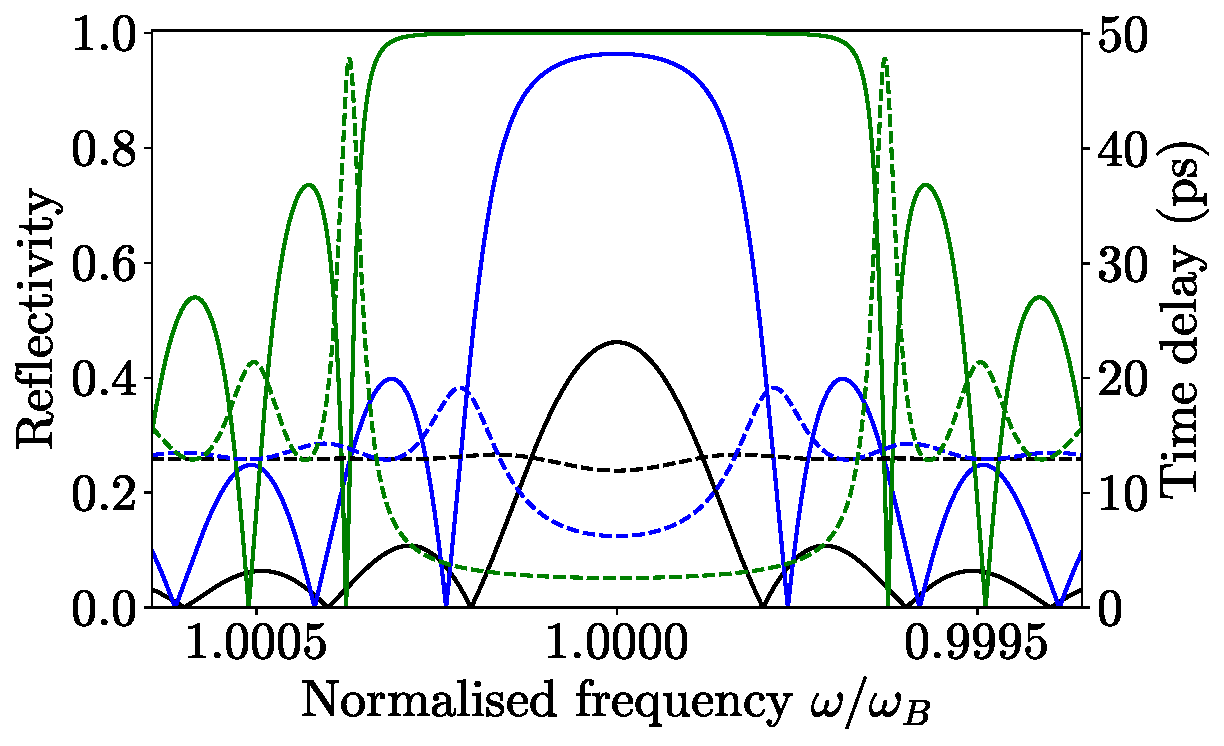
\includegraphics[width=\linewidth]{Images/Uniform_varying_kL_Rtau.pdf}
    \caption{Examples of aplitude reflectivity and group delay of uniform FBG reflection spectra with varying dimensionless grating strength $\k L_\text{FBG} \in [0.5, 2, 5]$ and constant number of grating periods $N=5000$.}
    \label{fig:uniform_spectra_varykL}
\end{figure}
%
\par
%
While varying $\kappa L_\text{FBG}$ suffices to illustrate the dependence on coupling strength without further substitutions, exploring changes in $\dnbar$ or $L_\text{FBG}$ requires expressing the frequency dependence explicitly.
Since $\kappa$ and $\hat{\sigma}$ depend only on wavelength and the prescribed grating parameters, the reflected amplitude $|\rho(\w)|$ and time delay can be directly plotted against frequency by substituting \eqref{eq:kappa} and \eqref{eq:sigma} into \eqref{eq:uniform_rho}.
Figure~\ref{fig:uniform_spectra_varyLdneff} shows examples of reflection spectra of uniform FBGs plotted against frequency, with the design frequency given by
%
\begin{equation}
    \w_D = \frac{\pi c}{\Lambda n_{eff}^2}
\end{equation}
%
highlighted to demonstrate the intrinsic shift of the Bragg resonance from the design frequency.
The reflection spectrum of a uniform grating has a maximum reflectivity
%
\begin{equation}
\label{eq:rmax}
    R \equiv |\rho_\text{max}| = \tanh{(\k L_\text{FBG})}
\end{equation}
%
centred at the Bragg frequency $\w_\text{max}$,
%
\begin{equation}
\label{eq:wBragg}
    \w_\text{max} = \frac{\w_D}{\left( 1 + \frac{\dnbar }{\neff}\right)}
\end{equation}
%
corresponding to the peak reflectivity.
We note that $R$ is more commonly used to denote reflected power rather than reflected amplitude; however, the present notation is adopted for clarity in later sections.
The first zeros on either side of the main lobe occur at $\w_\text{max} \pm \w_z$, where
%
\begin{equation}
\label{eq:wz}
    \w_z = \w_\text{max} \sqrt{\left( \frac{\dnbar}{2 \neff} \right)^2 + \frac{1}{N^2} }
\end{equation}
%
and the phase of the reflection spectrum shifts by $2\pi$ between these zeros.
Outside the main lobe, the reflectivity peaks of the side lobes decay exponentially, with a $\pi$ phase change across each sidelobe.
%
\begin{figure}[!t]
    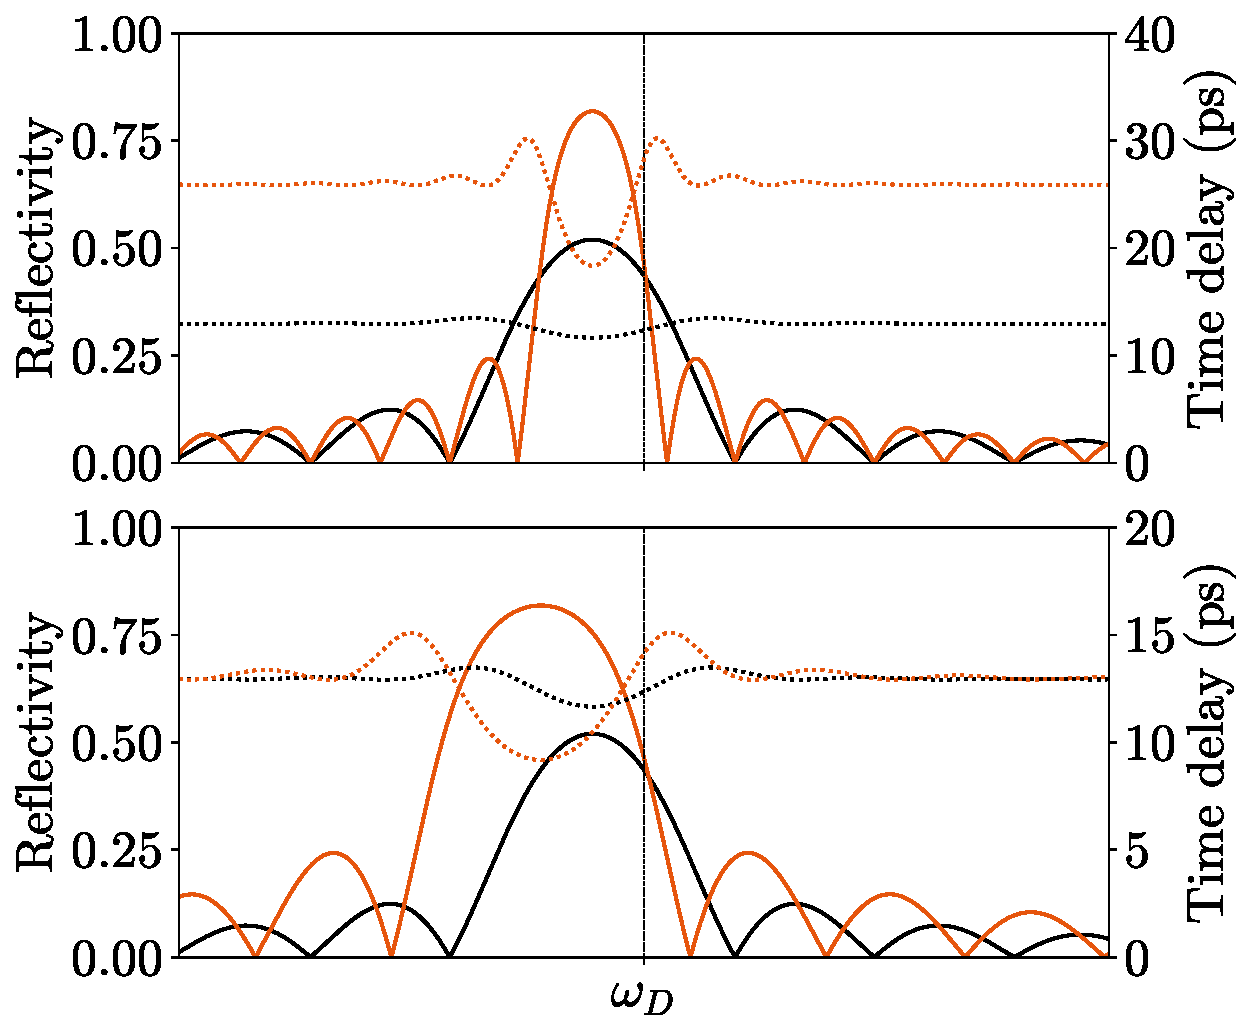
\includegraphics[width=\linewidth]{Images/Uniform_varying_L_dneff.pdf}
    \caption{Examples of the magnitude and group delay of uniform FBG reflection spectra, illustrating the effect of varying $\dnbar$ and $L_\text{FBG}$.
    The nominal case (black curves) corresponds to $\dnbar = 5\e{-5}\neff$ and $L_\text{FBG} = 2.64,\text{mm}$; in (a) the grating length is doubled to $L_\text{FBG} = 5.28,\text{mm}$, and in (b) the index change is doubled to $\dnbar = 1\e{-4}\neff$.}
    \label{fig:uniform_spectra_varyLdneff}
\end{figure}
%
\par
%
Figure~\ref{fig:uniform_spectra_varyLdneff}(a) shows that doubling $L_\text{FBG}$ increases $R$ because more grating periods contribute to reflection, reducing transmission.
At the same time, the bandwidth of each lobe is halved, while the shift of the reflection maximum from the design frequency remains unchanged.
In addition, the group delay is approximately doubled, since the light interacts with twice as many grating periods.
In contrast, doubling $\dnbar$, as shown in (b), again increases $R$, but now the shift from the Bragg resonance increases while the bandwidth remains unchanged.
The time delay is approximately the same between both cases, since the number of grating periods is unchanged.
Because these two parameters jointly determine the three key spectral features (resonance shift, maximum reflectivity, and bandwidth), it is not possible to vary one feature independently of the others.
Instead, a slight compensation to the grating period $\Lambda$ can be made, which shifts $\w_\text{max}$ while leaving $\wz$ and $R$ essentially unchanged.
This holds because laser centre frequencies are in the THz range, whereas the frequency offset is at most in GHz, so $\w_\text{max}/\w_D = \Lambda_D/\Lambda_\text{max} \approx 1$.
Using this approximation, together with \eqref{eq:wBragg} and \eqref{eq:wz}, $\dnbar$, $L_\text{FBG}$, and $\Lambda$ can be calculated sequentially using
%
\begin{align}
\label{eq:spec2phys}
    \dnbar &\approx \frac{2\wz}{\w_\text{max}} \frac{\neff}{\sqrt{1 + \left(\frac{\pi}{\arctanh{(R)}} \right)^2}},
    \\
    \Lambda &= \frac{\pi c}{\w_\text{max} \neff (\neff +\dnbar)},
    \\
    L &= \frac{\Lambda}{\sqrt{\left( \frac{\wz}{\w_\text{max}} \right)^2 - \left( \frac{\dnbar}{2\neff} \right)^2}}.
\end{align}
%
These expressions provide a direct inversion from spectral targets (bandwidth, reflectivity, and centre frequency) to physical grating parameters, enabling practical FBG design from desired optical specifications.
Taken together, these analytic results for uniform gratings provide the essential foundation for incorporating FBGs into feedback models of semiconductor lasers.
This framework links grating design directly to ECM structure and dynamics, setting the stage for analysing FBG feedback within the LK equations.
%
%
\section*{FBG distributed feedback}
\label{sec:FBG_feedback}
%
The spectral selectivity of FBGs, combined with their practical advantages already noted such as all-fibre integration, low insertion loss, and design flexibility, makes them especially well suited for FOF in semiconductor laser systems.
Building on the analytic understanding of uniform gratings, FBGs provide a direct route to reshaping the ECM structure in semiconductor lasers by tailoring their feedback spectrum.
This dual role, as practical devices and theoretical benchmarks, has motivated investigations of how FBG feedback modifies semiconductor laser dynamics within the LK framework.
A schematic of a semiconductor laser under external feedback from an FBG is shown in Figure~\ref{fig:FBG_setup}.
As discussed in \ref{subsubsec:FBG}, the reflection spectrum of an FBG can exhibit considerable complexity.
Since an FBG acts as a spectral filter, the feedback term $F(t)$ is given by \eqref{eq:FOF} with reflection spectrum $\rho(\w)$ given by \eqref{eq:uniform_rho}.
Equivalently, the feedback term can be expressed as a time-domain convolution,
%
\begin{equation}
    \label{eq:convolution}
     F(t) = e^{-i C_p} \tilde{\rho}(t) \otimes E(t-\tau)
\end{equation}
%
where $\tilde{\rho}(t)$ denotes the impulse response of the FBG relative to the Bragg resonance frequency.
Analytic expressions typically do not exist for the impulse response, even for simple gratings, and are therefore usually calculated numerically through fast Fourier transforms (FFTs), for example.
The need to compute $F(t)$ numerically restricts analysis to direct integration of the solutions $(E(t),N(t))$ and subsequent evaluation of time-series properties such as maximal Lyapunov exponents (MLEs) or spectral measures such as signal dispersion.
In contrast to the Lorentzian FOF case, no analytic reduction to a discrete DDE system has been proposed, making FBG feedback intrinsically more difficult to analyse.
Despite the substantial computational and analytical challenges posed by this feedback term, several studies have investigated uniform FBG feedback using the convolution representation for $F(t)$ given by \eqref{eq:convolution} \cite{li2012distributed, li2015chaotic, li2020stable, jiang2021characterizing, skenderas2021feedback, skenderas2024impact}.
%
\par
%
Early studies of FBG feedback relied mainly on numerical investigations, which provided limited analytic insight but revealed several important features of the resulting dynamics.
A primary motivation was the generation of broadband chaotic signals for applications such as high-speed optical random bit generation \cite{uchida2008fast} and chaos-based secure communication \cite{annovazzi2008secure}.
Compared with conventional mirror feedback, FBG feedback was shown to suppress the time-delay signature (TDS) much more effectively, thereby concealing the EC delay that autocorrelation-based attacks can exploit in encryption systems \cite{li2012distributed, jiang2021characterizing}.
This improvement was attributed to the distributed reflections along the FBG, which spread out the effective feedback delay.
Numerical studies demonstrated that TDS suppression improves as the FBG bandwidth decreases, owing to the stronger group-delay dispersion introduced by narrower gratings, while the FBG length plays little role in the suppression \cite{li2012distributed}.
However, this benefit comes with a trade-off: as the bandwidth narrows, the parameter regions supporting chaos shrink and are progressively replaced by stable period-1 oscillations \cite{li2020stable}.
Interestingly, FBG feedback can also generate chaos at shorter delays than mirror feedback, broadening the design space for compact devices \cite{li2012distributed}.
Beyond bandwidth effects, detuning between the laser frequency and the Bragg frequency plays a critical role: optimal TDS suppression occurs under positive detuning, consistent with the red-shift of the cavity resonance induced by the antiguidance effect \cite{li2015chaotic}.
Together, these results established FBG feedback as both a practical route to more secure chaotic carriers and a rich platform for exploring how spectral filtering reshapes external feedback laser dynamics.
%
\par
%
The convolution representation for $F(t)$ can also be expressed as a distributed delay term.
By definition,
\begin{equation*}
\tilde{\rho}(t) \otimes E(t-\tau) = \int_{-\infty}^{\infty} \tilde{\rho}(t-s) E(s-\tau)\,ds.
\end{equation*}
%
To render the integral finite, note first that $E(s-\tau) = 0$ for $s > t+\tau$, while the lower bound can be truncated at $t-T$, with $T$ chosen such that $\tilde{\rho}(s) \approx 0$ for all $s > T$, yielding an expression for $F(t)$ suitable for numerical integration
%
\begin{equation}
    \label{eq:distributed}
F(t) \approx e^{-i C_p} \int_{t-T}^{t+\tau} \tilde{\rho}(t-s) E(s-\tau)\,ds.
\end{equation}
%
This integral form highlights that FBG feedback acts as a weighted superposition of past fields, directly reflecting the spectral filtering imposed by the grating and contrasting with the single discrete delay characteristic of conventional optical feedback.
Both representations for $F(t)$ in \eqref{eq:convolution} and \eqref{eq:distributed} introduce numerical inaccuracies: truncation of the impulse response $\tilde{\rho}(t)$ limits the effective memory of the feedback, while discretisation of $\tilde{\rho}(t)$ or its frequency counterpart $\rho(\w)$ introduces sampling errors.
Such errors accumulate in the computation of the convolution or distributed-delay integral, setting practical limits on the accuracy of FBG feedback simulations.
%
\par
%
Motivated by the need for stronger dispersion to enhance TDS suppression, this distributed-delay formulation has also been applied to chirped fibre Bragg gratings (CFBGs) \cite{wang2017time, wang2019key, wang2023critical, chao2020permutation}.
Because analytic reflectivity spectra are unavailable for chirped gratings, \eqref{eq:wave_eqs} must be solved numerically, further increasing computational cost.
As in the uniform case, the impulse response $\tilde{\rho}(t)$ is obtained via FFTs and incorporated into the delay term.
Numerical studies demonstrated that CFBG feedback suppresses the TDS more effectively than uniform gratings and, in some cases, eliminates it entirely without requiring additional amplification, thereby simplifying experimental configurations.
In addition, the broader dispersion of CFBGs enriches the dynamical behaviour of the laser and expands the parameter space accessible for chaos-based applications, highlighting both the promise and the added complexity of chirped grating feedback compared to uniform designs.
%
\par
%
More recently, investigations have extended beyond the generation of chaotic signals, yet, as in earlier work, the use of the convolution representation for $F(t)$ has confined most studies to numerical integration of time series.
\Skenderas \textit{et al.} carried out a series of studies examining how detailed spectral features of FBGs impact semiconductor laser stability \cite{skenderas2021feedback, skenderas2022influence, skenderas2024impact}.
They showed that the positions of the zeros in the FBG reflection spectrum exert a strong influence on stability, with fluctuations emerging when these zeros overlap with the relaxation oscillation side lobes of the laser.
This effect was quantified by tracking the feedback rate required to trigger Hopf bifurcations for gratings of varying length (and thus bandwidth), highlighting that longer (narrower-band) gratings introduce stability oscillations even when overall reflectivity is kept constant.
An important observation was that detuning asymmetry, long observed in FBG feedback, was confirmed to be an intrinsic feature of the interaction between the spectral phase of the grating and the laser dynamics.
In later experimental work, they further demonstrated that small variations in the feedback phase, such as those induced by thermal tuning of the grating, can produce significant cyclic changes in stability, showing that both offset phase and phase fluctuations play a crucial role in shaping the dynamics \cite{skenderas2024impact}.
Overall, these studies show that while FBG feedback shares many broad features with filtered optical feedback, the detailed shape of the reflection spectrum—its zeros, side lobes, and phase—adds layers of complexity that strongly affect stability boundaries.
%
\par
%
While the convolution representation of $F(t)$ has provided limited insight into FBG feedback, no work has systematically analysed the external cavity mode (ECM) structure under FBG feedback, with the sole exception of studies by Naumenko \textit{et al.} \cite{naumenko2003characteristics,naumenko2004slow}
Their approach uniquely extended the analysis into the strong-feedback regime by adopting a multiple-reflection model, originally proposed for plain mirrors, and adapting it to the case of FBGs.
In this framework, the feedback term $\eta e^{-i C_p}E(t-\tau)$ in the LK equations is replaced by $E(t)\ln[E_r(t)/E(t)]$, where $E_r(t)$ represents the infinite series of external cavity reflections.
This reduces to the usual single-reflection term in the weak-feedback limit, but crucially retains the higher-order contributions required to capture the altered ECM structure when strong, frequency-selective feedback is present.
Here, the spectral filtering of the FBG enters explicitly through $\rho(\w)$, enabling the use of a Green-function formalism to derive stationary ECM conditions.
This provided, for the first time, a direct connection between the reflection spectrum of FBGs and the organisation of ECMs.
%
\par
%
Their results showed that, under weak feedback, ECMs remain largely confined to the main lobe of the FBG reflectivity, with the maximal gain mode (MGM) shifted close to the Bragg resonance frequency, reproducing the scenario found earlier for Lorentzian FOF.
As the FBG bandwidth narrows, however, new “satellite” ECM branches emerge, separated from the main ECM ellipse by the reflection zeros of the grating.
Under strong feedback, these satellites evolve into additional families of modes located within the side lobes of the FBG spectrum, fundamentally altering the accessible mode structure.
Follow-up investigations deepened these insights by examining dynamical consequences: the reshaped ECM structure could either suppress or destabilise low-frequency fluctuations depending on grating bandwidth and reflectivity, while intensity-noise studies revealed that strong FBG filtering not only generates new steady-state branches but also reshapes the balance between stable modes and antimodes.
%
\par
%
Together, these works demonstrate that an ECM-focused analytical treatment, rather than purely convolution-based time series simulation, provides unique insight into how FBG feedback reshapes both the topology and stability of the mode structure.
Yet, the complexity of the feedback term meant that full bifurcation analysis was not achieved, and these studies remain the only systematic attempt to connect the spectral features of FBGs—zeros, bandwidth, and side lobes—directly to the mode structure and noise properties of semiconductor lasers.
At the same time, the approach is computationally demanding: calculating ECMs requires solving intricate mode equations from the multiple-reflection expansion, while numerical integration is limited by both accuracy issues and long runtimes.
In addition, the formulation does not readily support advanced bifurcation tools such as numerical continuation, leaving the global organisation of solutions only partially characterised.
%
\par
%
Taken together, this review highlights the need for a modelling framework that unifies analytic tractability and numerical efficiency, something not achieved by current treatments of FBG feedback.
Ideally, such a model would preserve the physical accuracy of FBG feedback, yet remain mathematically tractable, yielding closed-form ECM conditions and enabling stability analysis available to existing filtered-feedback models.
At the same time, it should support efficient and accurate numerical integration, free from the heavy computational costs and accuracy concerns that currently constrain the current integro-differental equation formulations.
Developing such a framework would not only unify the fragmented perspectives on FBG feedback but also provide a practical tool for connecting grating design to laser dynamics in a transparent and predictive way.


% --- Summary of Introduction ---
% Semiconductor lasers are central to modern photonic technology, particularly in optical communications where their emission wavelengths align with network standards. Beyond their technological role, they also serve as paradigmatic systems for exploring nonlinear dynamics, since feedback turns their governing equations into delay differential equations (DDEs) with broad relevance across physics, engineering, and biology.
% External optical feedback (EOF) strongly shapes laser behaviour. The seminal Lang–Kobayashi (LK) equations first captured this by modelling a single-mode semiconductor laser under conventional optical feedback (COF) from a mirror. These equations revealed how external cavity modes (ECMs) emerge and interact, and their DDE structure allowed powerful analytical tools and numerical continuation to be applied. Since then, alternative feedback schemes have been explored. Phase-conjugate feedback (PCF) introduces symmetry that reorganises ECMs into isolated branches, while filtered optical feedback (FOF), especially with Lorentzian filters, has been studied in depth thanks to its analytic tractability. These studies showed that filtering reduces the number of ECMs, stabilises dynamics, and produces rich bifurcation structures, including codimension-2 and codimension-3 points that organise transitions in mode structure.
% Within this landscape, fibre Bragg gratings (FBGs) have attracted intense interest. They are all-fibre, low-loss, low-cost components whose reflectivity spectra can be precisely engineered. Uniform FBGs provide analytic solutions that serve as benchmarks, clarifying how reflectivity, bandwidth, and resonance shift depend on physical parameters. More advanced chirped FBGs (CFBGs) offer stronger dispersion and improved suppression of time-delay signatures (TDS), which is crucial for chaos-based communications. However, modelling feedback from FBGs poses challenges. Convolution- and distributed-delay formulations allow numerical time-series simulation but give only limited dynamical insight. Analyses of stability have shown roles for reflection zeros and detuning, but the mode structure itself has resisted systematic study.
% The one major exception is a series of works that extended ECM analysis to FBG feedback using a multiple-reflection framework. These studies demonstrated that spectral features of FBGs—zeros, side lobes, and bandwidth—directly reshape the ECM structure, creating new families of modes and altering noise properties. Yet this approach is computationally heavy, difficult to extend with bifurcation tools, and limited in scope.
% This review therefore highlights a critical gap: while existing models either enable analytic tractability (mirror and Lorentzian FOF) or capture physical realism (FBGs via convolution), no framework yet combines both. The field remains without a transparent, computationally efficient, and predictive model that can connect FBG design directly to laser dynamics while retaining compatibility with powerful DDE analysis tools.
% !TeX root = ../main.tex
\section{Uniform FBG modelling through discretised reflections}
\label{sec:FBG_discretised}
%
To overcome the limitations of convolution-based models and the absence of analytical ECM analyses, we seek a representation of FBG feedback that links directly to physical parameters while preserving the mathematically tractable delay–differential structure of the LK equations.
One promising route is to approximate the distributed reflection process directly in the time domain through discretised reflections.
Although most approaches in the literature begin with the spectral response of the grating, the reflection spectrum can also be modelled by approximating the grating as a sequence of discrete layers, each contributing a reflection and transmission event \cite{poladian2000simple, ghiringhelli2002time, feced2002efficient, skaar2001synthesis}.
This construction amounts to a discretised version of the impulse response $\tilde{\rho}(t)$ that would otherwise be obtained from $\rho(\omega)$ by an inverse Fourier transform.
By considering all optical paths that re-emerge from the FBG after a delay of $\tau_k$, the impulse response can be written as a weighted sum of delta functions,
%
\begin{equation}
    \label{eq:dicretised_impulse}
    \tilde{\rho}(t) = \sum_{k=0}^N h_r(k)\, \text{Dirac}(t-\tau-\tau_k)
\end{equation}
%
which we refer to as the discretised impulse response.
Physically, $h_r(k)$ encodes the effective amplitude of all paths contributing to the delayed signal emerging after a time delay $\tau_k$ as illustrated in Figure~\ref{fig:discretised_FBG}(a).
For non-uniform gratings, the average refractive index varies along the structure, requiring distinct refractive indices $n_i$ and corresponding transmission and reflection coefficients $t_{i,i+1}$ and $r_{i,i+1}$ to be computed for each layer.
This approach has been shown to recover the spectral response $\rho(\omega)$ with high accuracy \cite{ghiringhelli2002time}.
Here, however, we focus on the simpler case of uniform FBGs, where the average index is constant along the grating, so that all layers are identical.
This simplification yields a particularly transparent formulation of the feedback term $F(t)$ in terms of the coefficients $h_r(k)$, without requiring explicit reference to the full spectral response.
%
\par
%
We will show in the following that an approximate model for this discretised-reflection framework retains the analytic tractability of the Lorentzian FOF model discussed in section~\ref{subsec:FOF}, while also faithfully reproducing the reflection spectrum of uniform FBGs across a broad frequency range.
This combination of accuracy and simplicity opens the way to both closed-form equations for cavity modes, efficient numerical integration, and advanced numerical methods such as continuation.
%
%
\subsection{Uniform FBG discretised reflection model derivation}
\label{subsec:FBG_discretised_derivation}
%
\begin{figure}[!t]
    \centering
    
    \begin{overpic}[width=0.95\linewidth]{Images/discretised_reflections.pdf}
        \put(-1,60){(a)}
    \end{overpic}\\[0.5em]
    \begin{overpic}[width=0.95\linewidth]{Images/single_reflection_tk.pdf}
        \put(-1,60){(b)}
    \end{overpic}
    
    \caption{(a) Illustration of the first six layers in the slab decomposition of a uniform FBG, showing transmission and reflection coefficients between adjacent layers ($j=i+1$).
    (b) Illustration of the contribution to the reflected field arising solely from reflection at the $k^{\text{th}}$ layer, corresponding to the $k^{\text{th}}$ delayed signal.}
    
    \label{fig:discretised_FBG}
\end{figure}
%
\begin{figure}[!t]
    \centering
    
    \hspace{0.04cm}
    \begin{overpic}[width=\linewidth]{Images/R_tau_discretised_accuracy.pdf}
        \put(-4,93){(a)}
        \put(-4,48){(b)}
    \end{overpic}

    \caption{A comparison between the exact (solid lines) total reflection \eqref{eq:R_exact} and discretised (dashed lines) total reflection \eqref{eq:R_approx} is shown in (a), and the exact effective delay \eqref{eq:tau_exact} and discretised delay expectation \eqref{eq:tau_approx} is shown in (b) as functions of the normalised refractive index variation $\dn$ for varying $N \in [10,100,1000,10000]$.}

    \label{fig:R_approximations}
\end{figure}
%
We model the reflection response of a uniform FBG as arising from partial reflections at evenly spaced boundaries across $N$ layers of the grating.
The grating has a uniform average refractive index $\neff$, while each boundary introduces the same transmission coefficient $t$ and reflection coefficient $r$, determined by the normalised refractive index variation $\dn \equiv \dnbar/\neff$.
Further, the constant $\neff$ ensures that the round-trip time $\dt$ is constant across all layers so that $\tau_k = k \, \dt$.
For tractability, we consider only the dominant propagation paths that undergo a single reflection at the $(k-1)^\text{th}$ layer.
A contribution from such a path re-emerges from the grating after a time delay of $k\,\dt$, as sketched in Figure~\ref{fig:discretised_FBG}(b).
In this way, the discretised model mirrors the idea of an impulse response composed of delayed replicas of the input field, but expressed in terms of individual layer reflections.
%
\par
%
For the discretised formulation to be meaningful, it must reproduce the essential characteristics of a uniform FBG, most importantly the total reflectivity $R$, while linking the effective coefficients $r$ and $t$ to the physical parameters of the grating.
The exact reflectivity of a uniform FBG at its Bragg frequency, given by \eqref{eq:rmax}, can be written as
%
\begin{equation}
\label{eq:R_exact}
R_\text{exact} = \tanh{\left(\frac{\pi}{2}\frac{N \, \dn}{1+\dn} \right)}.
\end{equation}
%
A key observation is that this expression is very well approximated by the simpler form
%
\begin{equation}
\label{eq:R_approx}
R_\text{approx} = 1 - \left(1 - \dn \right)^{2N},
\end{equation}
%
as shown in Figure~\ref{fig:R_approximations}(a), where both forms are plotted as a function of $\dn$ for different $N$.
The close agreement confirms that the discretised model reproduces the correct scaling of reflectivity with both modulation depth and grating length.
To connect this approximation to a reflection model, we represent the signal emerging from the front facet after a time delay $k \, \dt$ as having passed through $k-1$ transmissive layers before being reflected at the $k^\text{th}$ layer, with no further attenuation thereafter.
The corresponding contribution is
%
\begin{equation}
\label{eq:hr1}
h_r(k) = t^{k-1} r,
\end{equation}
%
where $t$ and $r$ denote the effective transmission and reflection coefficients.
To ensure consistency with \eqref{eq:R_approx}, these coefficients must reproduce the total reflectivity when all delayed reflections are summed.
Rewriting \eqref{eq:R_approx} as a geometric series,
%
\begin{align*}
R_\text{approx} &= 1 - (1-\dn)^2 + (1-\dn)^2 - \dots \\
&\hspace{1em} - (1-\dn)^{2N-2} + (1-\dn)^{2N-2} - (1-\dn)^{2N} \\
&= \left( 1-(1-\dn)^2 \right)\left( 1 + (1-\dn)^2 + \dots + (1-\dn)^{2N-2} \right) \\
&= (1-(1-\dn)^2)\sum_{k=1}^{N} \left((1-\dn)^2\right)^{k-1},
\end{align*}
%
we arrive at an expression that is exactly reproduced by \eqref{eq:hr1} if we define
%
\begin{align}
\label{eq:tr}
t &\equiv (1-\dn)^2, \\
r &\equiv 1-(1-\dn)^2.
\end{align}
%
\par
%
Because FBGs act as distributed reflectors, it is not sufficient for the discretised model to match only the total reflectivity; it should also capture the effective delay of the structure, which represents how the reflected energy is distributed in time across multiple paths.
This can be tested by comparing the average delay predicted by the discrete reflections, $E[\tau_\text{FBG}]$, with the effective delay $\tau_{eff}$ derived directly from the exact reflection spectrum \cite{barmenkov2006effective}.
The effective time delay can be written in terms of the layer round-trip time $\dt = 2 \Lambda \neff/c$ as
%
\begin{equation}
    \label{eq:tau_exact}
    \tau_{eff} = \frac{R_\text{exact} \dt}{\pi \, \dn}.
\end{equation}
%
The expected delay of the discretised reflections $E[\tau_\text{FBG}]$ is calculated as the weighted average of the delays of all the reflected signals, where the weights are the amplitudes of the reflected signals.
Mathematically,
%
\begin{equation*}
    E[\tau_\text{FBG}] = \frac{r \sum_{k=1}^{N} t^{k-1} (k-1)\dt}{r \sum_{k=1}^{N} t^{k-1}}.
\end{equation*}
%
The sum in the denominator is simply the sum of a geometric sequence, having a closed form
%
\begin{equation*}
    \sum_{k=1}^{N} t^{k-1} = \frac{1-t^N}{1-t}.
\end{equation*}
%
The sum in the numerator can be evaluated efficiently by noting that it can be written in terms of a derivative w.r.t. $t$ of the numerator.
That is,
%
\begin{equation*}
    \sum_{k=1}^{N} t^{k-1} (k-1) = t \, \frac{\partial}{\partial t} \sum_{k=1}^{N} t^{k-1} = \frac{t(1-t^N)}{(1-t)^2} - \frac{N t^N}{1-t}.
\end{equation*}
%
The effective delay then simplifies to
%
\begin{equation}
    \label{eq:tau_approx}
    E[\tau_\text{FBG}] = \dt\left[ \frac{t}{1-t} - \frac{N t^N}{1-t^N} \right].
\end{equation}
%
\par
%
Figure~\ref{fig:R_approximations}(b) compares the effective delay $\tau_{eff}$ with the expected delay $E[\tau_\text{FBG}]$ of the discretised model, plotted as a function of $\dn$ for different $N$.
The comparison shows that the discretised model reproduces the effective delay with high accuracy, matching closely at small $\dn$ and diverging only gradually at larger values.
Although the accuracy of delay and reflectivity vary differently with $\dn$, the model reproduces both with sufficient consistency to remain reliable across the full parameter range.
%
\par
%
A key property of the coefficients in \eqref{eq:tr} is that they satisfy $r+t=1$, resembling the familiar balance between reflection and transmission.
Unlike true Fresnel coefficients, however, these are effective coefficients: they subsume the cumulative effect of multiple internal transmissions and reflections into a single pair of parameters.
In doing so, they preserve the correct scaling of reflectivity with $\dn$ and $N$ while providing a compact, physically transparent description that is straightforward to use in dynamical models such as the LK equations.
%
\begin{equation}
    \label{eq:discretised_impulse_full}
    \tilde{\rho}(t) = (1-t)\sum_{k=0}^{N-1} t^k \, \delta(t-\tau-k\dt)\, e^{-i k \wB \dt},
\end{equation}
%
where each term corresponds to a contribution that has traversed $k$ transmissive layers, been reflected once, and accumulated an additional phase $e^{-i k \wB \dt}$ from propagation through the grating.
Since the LK equations are defined relative to the free-running laser frequency (so that $\wZ=0$), the parameter $\wB$ naturally enters as the detuning of the grating's Bragg frequency.
This highlights that the FBG acts as a weighted superposition of delayed, phase-shifted replicas of the input field.
We remark that if backward transmission were explicitly included, alternative but mathematically consistent definitions of $r$ and $t$ could be derived, though the present choice yields cleaner expressions for the analysis that follows.
%
\par
%
With this foundation, the feedback term $F(t)$ follows directly as the convolution of the field with \eqref{eq:discretised_impulse_full}, consistent with earlier convolution-based formulations \cite{skenderas2024impact,skenderas2021feedback,li2012distributed,li2015chaotic,li2020stable}:
%
\begin{align*}
F(t) &= e^{-i C_p} E(t) \otimes \tilde{\rho}(t) \\
&\approx r e^{-i C_p} \sum_{k=0}^{N-1} t^k E(t) \otimes \delta(t-\tau-k\,\dt) e^{-i k \wB \dt} \\
F(t) &\approx (1-t) e^{-i C_p} \sum_{k=0}^{N-1} t^k E(t-\tau-k\,\dt) e^{-i k \wB \dt}.
\end{align*}
%
\par
%
Taken together, these results establish the discretised-reflection formulation as a reliable and practical approximation to FBG feedback.
Crucially, it preserves the analytic tractability of the LK system while embedding essential features of grating physics, thereby enabling both efficient time-domain simulations and deeper analytical exploration of cavity modes.
The central parameter $t$, which enters the LK equations, is determined directly from the target reflectivity via \eqref{eq:R_approx}:
%
\begin{equation}
\label{eq:discretised_t}
t = \big(1-R\big)^{1/N},
\end{equation}
%
providing a transparent connection between physical grating design and the discrete-feedback model.
This link ensures that the formulation is not only computationally convenient but also grounded in experimentally tunable parameters, making it a robust foundation for the analyses that follow.
%
\par
%
With both reflectivity and effective delay validated, the discretised model can now be embedded directly into the LK equations, which take the form
%
\begin{equation}
\label{eq:LK_discretised}
    \begin{aligned}
        \frac{d E}{d t} = (1 &+i \a) N(t) E(t) + \\
                        &\quad \eta (1-t) e^{-i C_p} \sum_{k=0}^{N-1} t^k E(t-\tau-k\, \dt) e^{-i k \wB \dt} \\
        T \frac{d N}{d t} &= P-N(t)-(1+2 N(t))|E(t)|^2.
    \end{aligned}
\end{equation}
%
Unlike convolution-based models, this formulation reduces the feedback to a finite sum of discrete delays, preserving the DDE structure for ECM analysis and continuation, while also providing a platform to explore the spectral properties of the system through its mode structure.
%
%
\subsection{EGM modes of the discretised reflection model}
\label{subsec:EGM_discretised}
%
A natural first step in assessing any feedback model is the calculation of its cavity modes, since these steady-state solutions provide the `backbone' of the system and reveal how the feedback reshapes the laser’s mode structure.
In the COF and FOF cases, mode calculations (ECMs and EFMs, respectively) have been central to validating both the physical realism and the analytical tractability of the models.
For the discretised FBG reflection model, the corresponding external grating modes (EGMs) serve the same purpose: they provide a direct spectral interpretation of the formulation, constitute the first point of comparison with the known reflection properties of uniform FBGs, and act as benchmarks for demonstrating that the model captures not only physical but also spectral characteristics of FBG feedback.
Beyond this role in validation, EGMs also structure much of the system’s dynamics and stability \cite{rottschafer2007ecm}, and once stable solutions are identified they can be systematically continued in parameters using specialised DDE continuation software such as \texttt{DDE-BifTool}.
%
\par
%
The EGMs take the form $(E(t), N(t)) = (E_s e^{i\w_s t}, N_s)$ with $E_s, \w_s, N_s \in \mathbb{R}$, corresponding to a laser field oscillating at a shifted frequency $\w_s$ with constant amplitude $E_s$ and inversion $N_s$.
Physically, $\w_s$ represents the detuning of the locked field from the solitary laser frequency $\w_0$.
Substituting this ansatz into \eqref{eq:LK_discretised} yields an implicit equation for the allowed EGM frequencies.
To this end, we first separate the resulting complex equation into its real and imaginary parts by expanding the exponentials, giving
%
\begin{align*}
    i \w_s = (1+i \a) N_s &+ \eta (1-t) \big(\cos{(\phi_\text{E})} -i\sin{(\phi_\text{E})}  \big) \times \\ 
                        &\left( \sum_{k=0}^{N-1} t^k \cos{(k\phi_\text{F})} - i \sum_{k=0}^{N-1} t^k \sin{(k\phi_\text{F})} \right)
\end{align*}
%
where $\phi_\text{F} = \dt(\wB + \w_s), \, \phi_\text{E} = C_p+\tau \w_s$ are the phases accumulated in the FBG and EC, respectively.
To evaluate the sums in closed form, we use the standard trigonometric series identities
%
\begin{align*}
    \sum_{k=0}^{N-1} &t^k \cos{(k\phi_\text{F})} = \\
    &   \frac{1 - t \cos{(\phi_\text{F})} - t^N \cos{(N\phi_\text{F})} + t^{N+1} \cos{((N-1)\phi_\text{F})}}{1 - 2t \cos{(\phi_\text{F})} + t^2} \\
    \sum_{k=0}^{N-1} &t^k \sin{(k\phi_\text{F})} = \\
    &\quad \quad \frac{t \sin{(\phi_\text{F})} - t^N \sin{(N\phi_\text{F})} + t^{N+1} \sin{((N-1)\phi_\text{F})}}{1 - 2t \cos{(\phi_\text{F})} + t^2}
\end{align*}
%
an implicit equation for the EGM frequencies $\w_s$ can be derived,
%
\begin{gather*}
    \begin{aligned}
\w_s = \frac{\eta (1-t) \sqrt{1 + \a^2}}{1 - 2 t  \cos{(\phi_\text{F})} + t^2} \times \\
&&\hspace{-6em} \Big[- &\sin{(\phi_\text{E} + \arctan\a)} \\
&&\hspace{-6em}      +  t&\sin{(\phi_\text{E} + \arctan\a - \phi_\text{F})} \\
&&\hspace{-6em}      + t^N&\sin{(\phi_\text{E} + \arctan\a + N \phi_\text{F})}   \\
&&\hspace{-6em}      -  t^{N+1}&\sin{(\phi_\text{E} + \arctan\a + (N-1) \phi_\text{F})}
\Big].
    \end{aligned}
\end{gather*}
%
After algebraic simplification, the right-hand side can be expressed as a single sine term, leading to
%
\begin{equation}
    \label{eq:discretised_ws}
    \w_s = -\eta (1-t) \sqrt{\a^2+1}\frac{S_N}{S} \sin{\left( \phi_\text{E}+\arctan\a + \Phi - \Phi_N  \right)}
\end{equation}
%
where
%
\begin{align}
    S &= \sqrt{1 - 2 t \cos{(\phi_\text{F})} + t^2}
    \\
    S_N &= \sqrt{1 - 2 t^N \cos{(N\phi_\text{F})} + t^{2N}}
    \\
    \Phi &= \arctan{\left( \frac{t \sin{(\phi_\text{F})}}{1 - t \cos{(\phi_\text{F})}} \right)} 
    \\
    \Phi_N &= \arctan{\left( \frac{t^N \sin{(N\phi_\text{F})}}{1 - t^N \cos{(N\phi_\text{F})}} \right)}.
\end{align}
%
We remark that in the plane mirror limit, the front face of the FBG would reflect all incoming light, that is $ t = 0 \implies S = S_N = 1, \, \Phi = \Phi_N = 0$, yielding 
%
\begin{equation*}
    \w_s = - \eta \sqrt{\a^2+1} \sin{(C_p + \w_s \tau + \arctan\a )}
\end{equation*}
%
which is precisely the well studied implicit ECM equation for the canonical COF case, validating the consistency of the derived equations \cite{rottschafer2007ecm}.
Given the solutions for $\w_s$, one can calculate $N_s$ and $E_s$ through
%
\begin{equation}
    N_s = -\eta (1-t) \frac{S_N}{S} \cos{\left( \phi_\text{E} + \Phi - \Phi_N \right)}  
\end{equation}
%
\begin{equation}
    E_s = \sqrt{\frac{P - N_s}{1 + 2 N_s}}
\end{equation}
%
The envelope of $f$, defined as $f_\text{env}(\w_s)$, is obtained by taking the extreme values of the sine term in \eqref{eq:discretised_ws}, i.e., setting it to $\pm 1$.
%
\begin{equation}
    \label{eq:discretised_ws_envelope}
    f_\text{env}(\w_s) = \mp \eta (1-t) \sqrt{\a^2+1}\frac{S_N}{S}
\end{equation}
%
Moreover, by substituting the CW ansatz back into \eqref{eq:LK_discretised}, one obtains an explicit expression for $N_s(\w_s)$, given by
%
\begin{gather}
    \label{eq:discretised_Ns_curve}
    \begin{aligned}
        \hspace{-0.5em}N_s(\w_s) = &\frac{\a \w_s}{1+\a^2} \pm \\
                    &\frac{1}{1+\a^2}\sqrt{-\w_s^2 + (1+\a^2) \left(\eta (1-t) \frac{S_N}{S} \right)^2}.
    \end{aligned}
\end{gather}
%
Finally, while the grating’s reflectivity and detuning are controlled through $\eta$ (or $R$) and $\wB$, respectively, the number of layers $N$ provides an additional design parameter, directly setting the FBG bandwidth $\wz$ via \eqref{eq:wz} and \eqref{eq:R_approx}.
%
\begin{equation}
    \label{eq:wztoN}
    \wz = \w_\text{max} \sqrt{\left( \frac{1 - (1 - R)^\frac{1}{2N}}{2} \right)^2 + \frac{1}{N^2}}
\end{equation}
%
\begin{figure}[!t]
    \centering 
    
    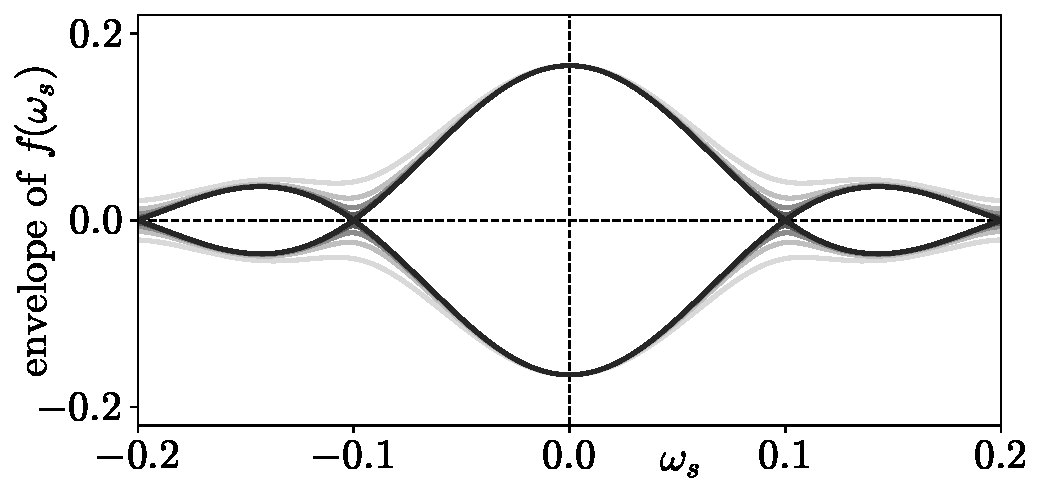
\includegraphics[width=\linewidth]{Images/discretised_EGM_envelope_variations.pdf}   
    
    \caption{Variation in the shape of the envelope $f_\text{env}(\w_s)$ for $R \in [0.01, 0.2, 0.4, 0.6, 0.8]$ while keeping the effective feedback rate $\eta R$ constant.}
    
    \label{fig:discretised_EGM_envelope_variations}
\end{figure}
%
\begin{figure}[!t]
    \centering
    \hspace{1em}
    \begin{overpic}[width=0.9\linewidth]{Images/Low_N_gratings.pdf}
        \put(-5,54){(a)}
    \end{overpic} \\
    \vspace{1em}
    \begin{overpic}[width=\linewidth]{Images/discretised_EGM_varyN.pdf}
        \put(0,82){(b)}
        \put(0,40){(c)}
    \end{overpic}  \\
    \vspace{1em}
    \makebox[\linewidth][c]{%
    \hspace{1em}%
    \begin{overpic}[width=0.99\linewidth]{Images/discretised_EGM_wideview.pdf}
        \put(-1,42){(d)}
    \end{overpic}%
    }
    \caption{(a) Illustrations of gratings with equal length but different layer numbers $N$.
    (b), (c) Equivalence in EGM structure between different grating numbers $N \in [10, 22500]$ by keeping $N\dt$ constant, each providing near identical reflection zero locations $\wB \pm n\wz, \; n \in \mathbb{N}$.
    EGM frequencies $\w_s$ are intersections of $f(\w_s)$ (blue curve) and $g(\w_s)$ (green curve) in (a), while the envelope $f_\text{env}$, consisting of two curves is in black.
    The EGM solutions and their curve in the $(\w_s, N_s)$-plane are shown in (b).
    The red dots correspond to a discrete set of EGMs, where modes are indicated with circles while antimodes are indicates by squares.
    The black curve connecting the the set of EGMs is given by \eqref{eq:discretised_Ns_curve}.
    (d) EGM solutions over a wide frequency range $\w_s \in [-20\wz, 20\wz]$.
    In panels (b)–(d), results for $N=10$ are plotted in lighter shades, while results for $N=22500$ are plotted in darker shades.
    }

    \label{fig:discretised_EGM_varyN}
\end{figure}
%
\begin{figure*}[!t]
    \flushleft
    \hspace{1em}
    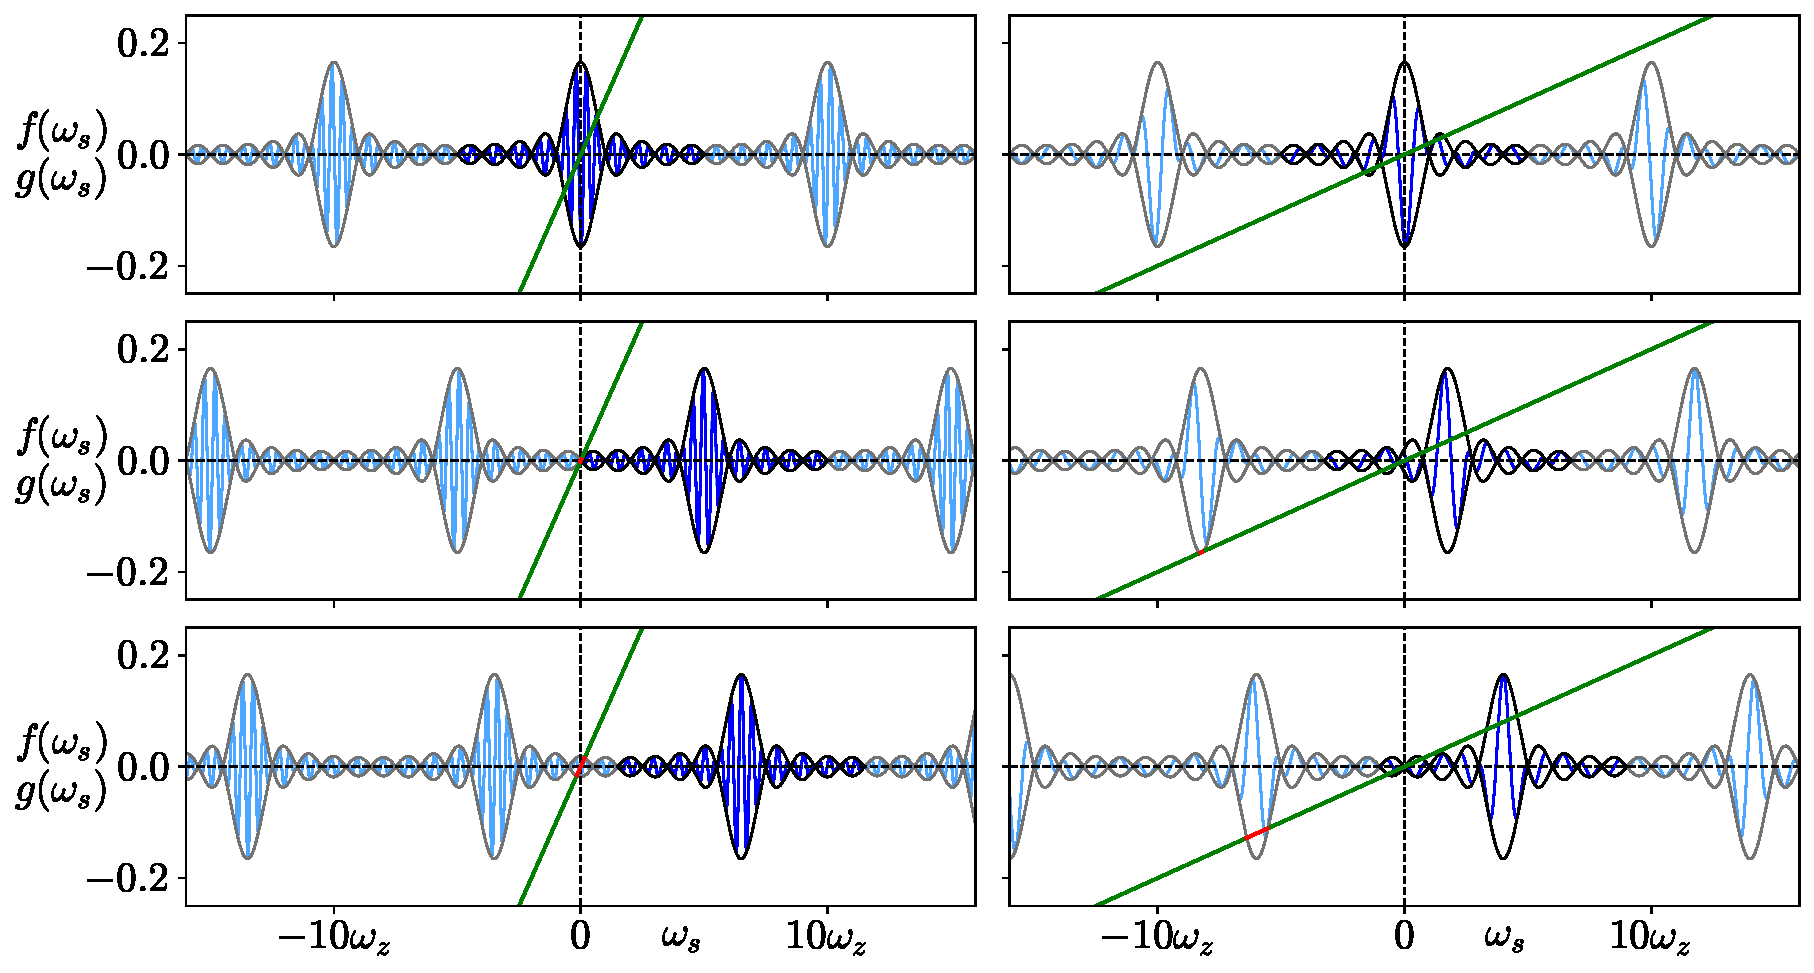
\includegraphics[width=0.87\linewidth]{Images/discretised_EGM_minimumN.pdf}
    
    \caption{EGM solutions for varying detuning $\wB$ with $\wz=0.1$ (left) and $\wz=0.02$ (right) and $N=10$ in both cases.
    Valid region solution regions correspding to the frequency range $\wB \pm 5 \wz$ are plotted with opaque lines while the entire frequency region is plotted with semi transparent lines.}
    
    \label{fig:discretised_EGM_minimumN}
\end{figure*}
%
\par
%
At this point, the EGM equations allow us to directly visualise the spectral structure predicted by the discretised reflection model.
In particular, the solution envelope $f_\text{env}(\w_s)$ provides a direct analogue of the FBG reflection spectrum, just as the envelope in the FOF case recovers a Lorentzian profile \cite{green2006mode}, while the envelope in the COF case being flat (and thus frequency indepedent) \cite{rottschafer2007ecm}.
This makes it a natural diagnostic for selecting the effective grating parameters $(R, N, \dt)$.
To anchor the discussion, we fix the laser and EC parameters to the canonical values $\tau = 121, \a = 3.5, \eta R = 0.0455, C_p = 0, T = 550, P = 0.186$ \cite{heil2003delay,krauskopf2004dynamics}, and prescribe a grating bandwidth $\wz = 0.1$ with detuning $\wB=0$.
For 1550 nm light, this choice of $\wz$ corresponds to $N \approx 22500$ layers (see Appendix~\ref{app:LK_nondim} for details).
%
\par
%
We first examine how the envelope changes with reflectivity $R$ while keeping the product $\eta R$ fixed.
As shown in Figure~\ref{fig:discretised_EGM_envelope_variations}, well-resolved transmission zeros at $\w_s = \wB \pm n\wz$ emerge only when $R$ is small.
This motivates adopting the practically relevant limit $R\ll1$, in which $\eta$ is rescaled so that the effective feedback rate $\eta_\text{eff} \equiv \eta R$ remains fixed.
In this regime, \eqref{eq:wztoN} simplifies to
%
\begin{equation}
\label{eq:wz_approx}
\wz \approx \frac{2\pi}{N \dt},
\end{equation}
%
so that the bandwidth is controlled entirely by the product $N\dt$, or equivalently, by the physical grating length $L = N \dt c/\neff$.
%
\par
%
This simplification provides a powerful degree of freedom: $N$ can be reduced substantially without altering the envelope spectrum, provided $N\dt$ is kept constant.
Figure~\ref{fig:discretised_EGM_varyN}(b) illustrates this invariance, showing near-identical envelopes for gratings with $N$ ranging from $10$ to $22500$ once $N\dt$ is matched.
Physically, this reflects the intuition that short gratings behave as broadband reflectors, while longer gratings act as narrowband filters.
The ability to tune $N$ while preserving the spectral response means the model can be kept numerically tractable for continuation and integration.
%
\par
%
Beyond the excellent agreement in the envelopes $f_\text{env}(\w_s)$ for drastically different $N$, Figure~\ref{fig:discretised_EGM_varyN}(a) additionally illustrates the strong agreement between the curves $f(\w_s)$ and $g(\w_s)$, defined as as the left- and right-handside of \eqref{eq:discretised_ws}, respectively.
In the standard way, EGM solutions visualised in the $(\w_s, N_s)$-plane in (b) are found numerically by the intersections $f(\w_s)$ and $g(\w_s)$ shown in (a) and mirror the excellent agreement already demonstrated with the solution envelopes.
In this case, the EGMs lie within the main lobe on the closed curve given by \eqref{eq:discretised_Ns_curve} with modes (stable EGMs) indicated by circles lying on the lower portion of the curve and anti-modes (unstable EGMs) indicated by squares lying on the upper portion of the curve.
It is noted that agreement in the solutions degrades for EGMs with larger frequency detunings $\w_s$, although the agreement is still reasonable for practical purposes.
We therefore may select a layer number $N$ that is low enough to be amenable to standard numerical analyses such as continuation without encountering significant computational difficulties.
%
\par
%
The main practical consequence of working with a reduced grating number $N$ is that only a limited number of side lobes are reproduced accurately.
Figure~\ref{fig:discretised_EGM_varyN}(d) illustrates this by plotting the curves $f(\w_s)$ and $f_\text{env}(\w_s)$ over $\w_s \in [-20\wz,20\wz]$ for $N=10$ and $N=22500$ with $N\dt$ fixed.
When $N=10$, the envelope repeats after every $10\wz$, so that only five side lobes are physically meaningful before the spectrum develops unphysical repetitions.
By contrast, the $N=22500$ case reproduces the correct extended sequence of side lobes expected from a uniform FBG.
This highlights the need to choose $N$ small enough to keep the model tractable, but large enough to capture all features relevant to the parameter ranges under study.
%
\par
%
Figure~\ref{fig:discretised_EGM_minimumN} shows two specific artefacts that arise if $N$ is taken too small, allowing a lower bound on $N$ to be derived.
The first is a detuning-induced loss of validity: as $\wB$ increases, the valid spectral window of width $\pm 5\wz$ can shift away from $\w_s=0$, and beyond this range the repeated envelope begins to grow again, which is unphysical.
This can be avoided by requiring $N > 2|\wB|_{\max}/\w_{z,\min}$.
The second artefact is the appearance of spurious intersections when repeated main lobes cross the line $f(\w_s)=\w_s$, creating artificial EGM branches.
The first repetitions of the main lobe occur at $\w_s = \pm N\wz + \wB$, while the envelope reaches extrema at $\pm \eta\sqrt{1+\a^2}$.
To prevent such intersections, one must ensure that $N\wz + |\wB| > \eta\sqrt{1+\a^2}$.
Taken together, these two requirements provide a practical lower bound for the grating number:
%
\begin{equation}
    \label{eq:Nmin}
    N_\text{min} =
    \begin{cases}
    \left\lceil \dfrac{2|\wB|_{\max}}{\w_{z,\min}} \right\rceil, \; |\wB|_{\max} > \eta_{\max}\sqrt{1+\a_{\max}^2}, \\[2ex]
    \left\lceil \dfrac{|\wB|_{\max} + \eta_{\max}\sqrt{1+\a_{\max}^2}}{\w_{z,\min}} \right\rceil, \; \text{otherwise}.
    \end{cases}
\end{equation}
%
With these conditions satisfied, the discretised model remains spectrally faithful while retaining the low dimensionality needed for efficient continuation and simulation.
%
\par
%
Taken together, these observations show that the EGM envelope both recovers the expected reflection spectrum and guides the principled choice of grating parameters.
Small $R$ ensures accurate reflection zeros, the product $N\dt$ fixes the bandwidth, and the lower bound in \eqref{eq:Nmin} guarantees physical side-lobe structure.
With these conditions, the discretised model remains both spectrally faithful and computationally manageable.
% !TeX root = ../main.tex
\section{Comparison to previously studied FBG feedback models}
\label{sec:model_comparison}
%
Given the excellent agreement in ECMs confined to the main lobe between the three Lorentzian model and the discretised reflection model, we now compare agreement in solution structure and system dynamics between the discretised reflection model and the various approaches to modelling the feedback term $F(t)$ within the LK equations in the literature. This section demonstrates the excellent agreement this discretised model demonstrates with significantly less computational effort, while portraying several analysis techniques available to this system that is not possible with previously studied forms of FBG feedback. 
%
%
\subsection{EGM Accuracy}
\label{subsec:naumenko}
A considerably more complex system presented by Naumenko \textit{et al.} in \cite{naumenko2003characteristics} considers the feedback term $F(t)$ in the form of \eqref{eq:multiple_EC} that is, as the inverse Fourier transform of the product of the time delayed electric field in the spectral domain $\mathcal{F}[E(t-\tau)](\w)$ and the grating reflection spectrum $\rho(\w)$. The model additionally considers nonlinear gain and frequency chirp due to thermal effects when the injection current is changed. Ignoring these additional effects, and making suitable approximations, the system simplifies to the derived discretised reflection system as shown in Appendix~\ref{sec:multiple_EC_nondim} with parameter values $(\a, P, T, \tau, C_p) = (4, 0.5, 123, 512, 0)$, and varying grating parameters $\eta$, $\wB$, and $\wz$.
%
\par
%
EGMs were calculated with the help of Green functions through an involved mathematical procedure, as opposed to deriving closed form analytical equations. As discussed in the introduction, they identified `satellite' EGMs, separated from the central EGM envelope by the zeros of the main lobe by varying both grating bandwidth $\wz$ and detuning $\wB$.
%
\begin{figure}[!t]
    \centering

        \begin{overpic}[width=0.74\linewidth]{Images/rB_003_annotated.pdf}
            \put(-2,44){(b)}
            \put(-2,96){(a)}
        \end{overpic}\\
        \hspace{-2.2em}
        \begin{overpic}[width=0.65\linewidth]{Images/Naumenko_EGM_rB003.pdf}
            \put(-5,80){(c)}
        \end{overpic}

    \caption{A comparison between EGMs in the multiple reflection (left) and discretised FBG (right) models in the frequency-intensity domain for varying grating bandwidth and zero detuning. 
    The curves in panels (a1) and (a2) illustrate the FBG frequency responses. 
    A constant reflectivity of $R=0.0316$ yields a nondimensionalised effective feedback rate $\eta=0.085$ while Bragg grating reflection zeros at 1/3, 4/3, and 20/3 GHz yield nondimensionalised reflection zero locations $\wz=0.016\pi, \; 0.064\pi, \; 0.32\pi$. 
    The EGMs in panels (b1) and (b2) corresponding to these respective bandwidths are plotted with circles $(\circ)$, diamonds $(\diamond)$ and squares $(\square)$, while the MGM in each case is plotted indicated by a $\times$.}
    
    \label{fig:Naumenko_rB003}
\end{figure}
%
\begin{figure}[!t]
    \centering

    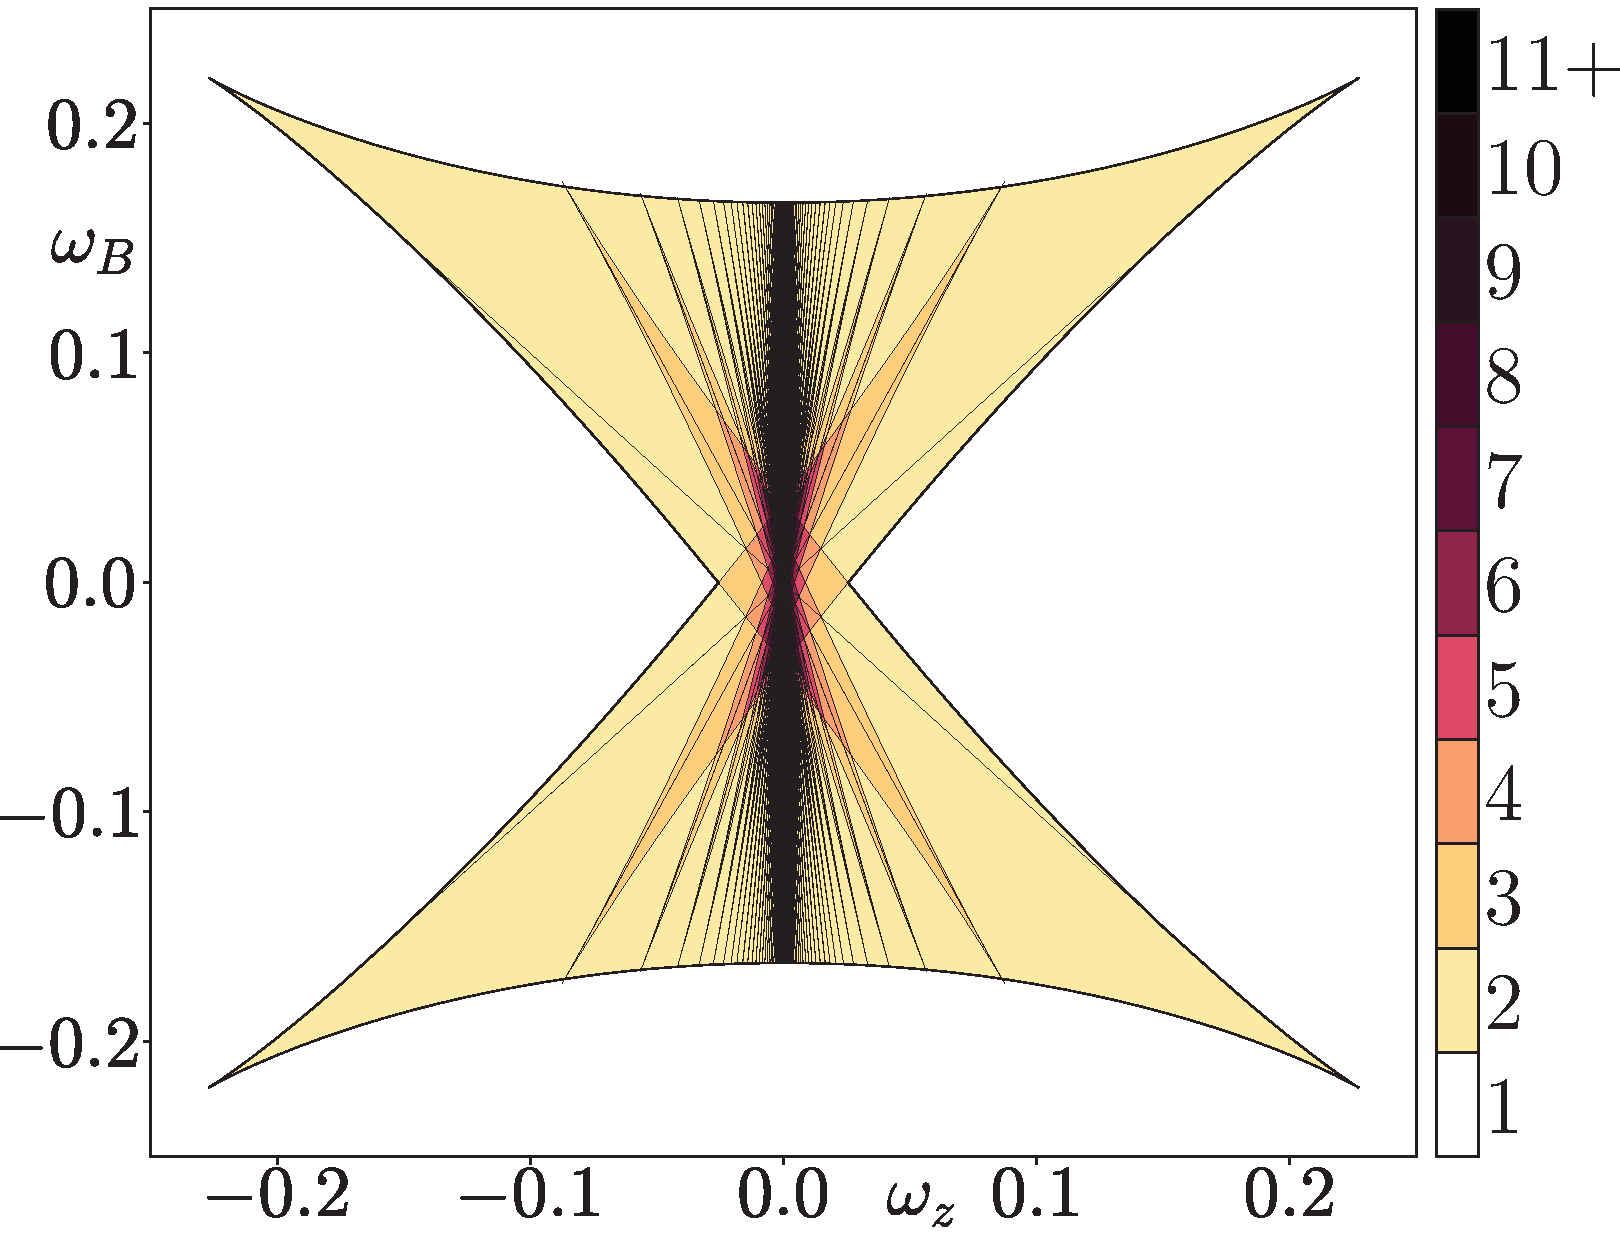
\includegraphics[width=\linewidth]{Images/EGM_components_2D_coloured.pdf}

    \caption{Caption.}
    
    \label{fig:EGM_components}
\end{figure}
%
Figure~\ref{fig:Naumenko_rB003} compare results obtained by both the multiple EC reflection FBG feedback and discretised FBG models for varying grating reflectivity, bandwidth and detuning. 
In order to to obtain valid EGM solutions, for both parameter sets, $N=10 > N_\text{min}=7$ was used. 
Solutions are projected in the frequency-intensity plane where $I = |E|^2$, in contrast to the usual projection in the inversion-frequency plane, causing an inversion of the cavity modes about the frequency axis. 
The photon lifetime $\tau_p=24\,\text{ps}$ was used to convert grating bandwidths in Hz to their nondimensionalised $\wz$ form. 
Clearly, excellent agreement in the mode structure is achieved, in particular for the low feedback rate case. 
Firstly, considering no detuning, low feedback and varying bandwidths as is the case in Figure~\ref{fig:Naumenko_rB003}, 
for a wide bandwidth of the Bragg reflector (in this case, a main lobe width of 40/3 GHz or $2\wz=0.64\pi$ in nondimensionalised form), EGMs lie on a closed curve, resembling a COF ECM structure, as expected. 
The MGM (mode with highest power) is located for near the edge of the left side of the closed curve, indicated by an '$\times$' in the figure. 
As the FBG bandwidth is decreased, the number of EGMs decreases, and the EGM solution curve and MGM narrows as they are confined to within the bandwidth of the main lobe, 
in agreement with results obtained from Sections~\ref{sec:EGM_Lorentzian} and \ref{sec:EGM_discretised} and with results obtained for a single Lorentzian filter \cite{yousefi1999dynamical}. 
Further narrowing the filter bandwidth introduces satellite EGMs, indicated with triangles, due to the side lobes of the FBG reflection spectrum. 
It is noted that this effect does not occur in the single Lorentzian filter for zero detuning. 
At this point, the MGM as nearly at the Bragg frequency, in agreement with physical intuition. 
Increasing the feedback rate considerably, and detuning the FBG from the laser's free-running frequency, as shown in Figure~\ref{fig:Naumenko_rB02}, 
also detune the EGM modes, and split the modes into three disjoint curves, corresponding to the main lobe and two side lobes nearest to the laser's free-running frequency. 
This splitting of solution curves was similarly observed for the single Lorentzian filter \cite{yousefi1999dynamical}, but at most two disjoint curves can be formed \cite{green2006mode}, while in this case already three distinct solution curves are present. 
Significant distortion in the EGM structure along the intensity axis can be seen for the discretised reflection case compared to the Multiple EC reflection model, 
which can be attributed to the lack of a gain suppression factor in this model in this simplified model. 
In any case, excellent agreement in the locations of the EGM components, MGM, and number of EGM solutions demonstrates the ability of the discretised reflections model to capture the solution structure of FBG feedback.
%
\par
%
\subsection{Stability Fluctuations}
\label{subsec:lichaos_skenderas}
%
\begin{figure}[t]
    
    \begin{overpic}[width=0.9\linewidth]{Images/Reflection_zero_overlap.pdf}
        \put(2,86){(a)}
        \put(2,43){(b)}
    \end{overpic}

    \caption{Caption}
    
    \label{fig:zero_overlap}
\end{figure}
%
It is important to note that while the locations of zeros in the discretised model are uniform, is only the case for FBGs which have relatively low reflectivities, see Figure~\ref{fig:uniform_spectra_varykL}. 
For this, re 
%

\begin{figure}[t]
    \flushleft
    \begin{overpic}[width=0.845\linewidth]{Images/Li_chaos_heatmap_image.pdf}
        \put(-2,77){(a)}
    \end{overpic}\\
    \vspace{-0.5em}
    \begin{overpic}[width=0.99\linewidth]{Images/discretised_Lichoatic_wBeta_comparison_hopfs_minbifs_ai.pdf}
        \put(-2,65){(b)}
    \end{overpic}\\
    \vspace{-0.5em}
    \begin{overpic}[width=\linewidth]{Images/discretised_Lichoatic_wBeta_comparison_lyapunovs.pdf}
        \put(-2,70){(c)}
    \end{overpic}

    \caption{Comparison between two parameter dynamical mappings of output intensity for a convolved FBG feedback form of $F(t)$ \cite{li2012distributed,li2015chaotic,li2020stable} (a) 
    and the discretised FBG feedback form of $F(t)$ in the parameter space of feedback strength ($\xi_f$ in (a) and equivalent $\eta$ in (b)) 
    and grating detuning frequency ($\Delta f$). 
    In (a), the laser output intensity is stable (white), period-one oscillatory (red), quasi-periodic pulsating (gray), period-doubled oscillatory (yellow), and chaotic (black). 
    In (b), the laser output is in steady-state (white), period-one oscillatory (red), period-two (yellow), and period 3 to very large period in a gradient from grey to black. 
    In (c) parameter sweeps are performed in all four directions, with Hopf bifurcations of steady state EGMs overlayed.}
    
    \label{fig:Li_chaos}
\end{figure}
%
\par
%
Finally, we compare our model to the most recent work on semiconductor lasers under FBG feedback by \Skenderas \textit{ et al.} \cite{skenderas2021feedback,skenderas2024impact}. 
In contrast to the previous two models, where nondimensionalisations and approximations were required before direct comparisons could be made, the form of the equations analysed mirror the equations presented in this work, 
using parameter values $(\a, P, T, \tau) = (3, 1, 1000, 1000)$, except for the use of a convolution feedback term $F(t)$ of the form \eqref{eq:convolution}. 
The results presented by \Skenderas \textit{ et al.} therefore serve as the most suitable basis for comparisons in the accuracy of the derived discretised model. 
Given the complexity of analysing the LK equations under FBG feedback using a convolution term, the results presented, 
like those previously studied, are obtained solely through analysis of time series obtained through numerical integration. 
The main focus of their analysis is in characterising the interplay between the lasers relaxation oscillations (ROs) and the FBG reflection zeros as a function of feedback rate $\eta$ and grating bandwidth $\wz$ for varying feedback phase $C_p$ and grating detuning $\omega_B$. 
%
\par
%
ROs are the most typical type of oscillation that one would expect in semiconductor lasers. 
They are damped intensity fluctuations that occur when the laser transitions between steady states, typically after a sudden change in injection current, 
and arise from the dynamic interplay between photon density and carrier density in the laser cavity. 
When the carrier population is perturbed, it overshoots the steady-state value, causing oscillations in output power at a characteristic frequency known as the relaxation oscillation frequency $\w_\text{RO}=\sqrt{2P/T}$, 
which form the dominant side lobes either side of the centre frequency in the Fourier spectrum of a semiconductor laser. 
Exciting the ROs of a laser can lead to a more unstable laser, and therefore one would expect that lower amount of feedback would cause the laser to transition from steady output to oscillatory and then more unstable outputs. 
%
\par
%
The strategy employed by the authors to observe this behaviour is by tracking the Hopf bifurcation of the steady state of the laser in the $(L_\text{FBG},\eta)$-plane, 
where the grating length $L_\text{FBG}$ can be used to control the grating bandwidth $\wz$ as discussed in \ref{sec:EGM_discretised}. 
As discussed in \ref{sec:FBG}, varying the grating length also changes the grating reflectivity, therefore, when using this model, grating parameters must be simultaneously varied to solely vary its bandwidth. 
This is not an issue with the discretised reflections model as bandwidth $\wz$ and thus length $L_\text{FBG}$ can be varied independent of reflectivity using \ref{eq:wz_approx}
%
\begin{equation}
    L [\text{m}] \approx \frac{\pi c \tau_p}{\wz \neff} 
\end{equation}
%
where $\tau_p$ is the photon lifetime used to rescale time in this form of the LK equations as discussed in Section~\ref{sec:EGM_discretised}.
%
\par
%
\begin{figure}[!t]
    \flushright
    \begin{overpic}[width=\linewidth]{Images/discretised_Skenderas_wzeta_Cpcomparison_N20.pdf}
        \put(-3,55){(a)}
    \end{overpic}\\
    \hspace{-0.5em}
    \begin{overpic}[width=0.98\linewidth]{Images/discretised_Skenderas_wBeta_image.pdf}
        \put(-3,75){(b)}
    \end{overpic}\\
    \hspace{-0.5em}
    \begin{overpic}[width=0.97\linewidth]{Images/discretised_Skenderas_wBeta_comparison_minbifs_ai.pdf}
        \put(-3,75){(c)}
    \end{overpic}

    \caption{The evolution of Hopf bifurcation tracking the stability fluctuations as a function of $L_\text{FBG}$ at zero detuning for different values of the feedback offset phase $C_p$ equal to 
    $0$ (blue), $\pi /4$ (yellow), $\pi/2$ (violet), $2\pi/3$ (green), $\pi$ (cyan), $3\pi/2$ (maroon), and $7\pi/4$ (orange). Comparison between two parameter dynamical mappings of output intensity for a convolved FBG feedback form of $F(t)$ \cite{li2012distributed,li2015chaotic,li2020stable} (a) 
    and the discretised FBG feedback form of $F(t)$ in the parameter space of feedback strength ($\xi_f$ in (a) and equivalent $\eta$ in (b)) and grating detuning frequency ($\Delta f$). 
    In (a), the laser output intensity is stable (white), period-one oscillatory (red), quasi-periodic pulsating (gray), period-doubled oscillatory (yellow), and chaotic (black). 
    In (b), the laser output is in steady-state (white), period-one oscillatory (red), period-two (yellow), and period 3 to very large period in a gradient from grey to black. 
    In (c) parameter sweeps are performed in all four directions, with Hopf bifurcations of steady state EGMs overlayed}
    
    \label{fig:Skenderas_wBeta}
\end{figure}
%


% !TeX root = ../main.tex
\section*{Conclusions and future developments}
\label{sec:conclusions}%
While a low reflectivity $R$ does provide the desired transmission zeros, the relative errors in both total reflectivity $R_\text{error}$ and delay $\tau_\text{error}$ are larger compared to larger total reflectivities. 
This is demonstrated in Figure~\ref{fig:NR_Selection}, which visualises the combined relative errors $R_\text{error}$ and $\tau_\text{error}$ using the Euclidean metric $\| R_\text{error}, \tau_\text{error} \|_{_2} = \sqrt{R_\text{error}^2 + \tau_\text{error}^2}$. 
For the choice $N=10$, a total reflectivity $R_\text{approx} = 0.75$ would provide a lower combined error of 4\% as shown in (a) compared to the $R_\text{approx} = 0.1$ which has a combined error of 19\%. 
As the ability to effectively describe and analyse transmission zeros of FBGs is of great interest, this increase in combined error, which is still relatively low from a modelling perspective, is a an acceptable trade-off.
%
\begin{figure}
    \centering
    
    \includegraphics[width=\linewidth]{Images/NR_Selection.pdf}
    
    \caption{Combined relative errors of FBG total reflectivity $R_\text{error}$ and delay $\tau_\text{error}$ as a function of the grating number $N$ and normalised refractive index variation $\dn$. 
    Level sets of constant total reflectivity $R_\text{approx}$ are overlayed in white. 
    In (a), the square marker at $(N,\dn) = (10, 0.07)$, corresponding to an $R_\text{approx} = 0.75$ has a combined error of 4\% while in (b), the marker at $(N,\dn) = (10, 0.0055)$, 
    corresponding to an $R_\text{approx} = 0.1$ has a combined error of 19\%.}
    
    \label{fig:NR_Selection}
\end{figure}
%

% =======================
% Acknowledgments (optional)
% =======================
\begin{acknowledgments}
We acknowledge ...
\end{acknowledgments}

% =======================
% Appendices (optional, modular)
% =======================
\appendix
% !TeX root = ../main.tex
\section{Nondimensionalisation of the original LK Equations}
\label{app:LK_nondim}
%
\let\cleardoublepage\origcleardoublepage
%
To model the dynamics of a semiconductor laser with optical feedback from an external cavity, we use the well-known \textbf{Lang-Kobayashi equations} \cite{lang1980external}. These delay differential equations describe how the complex electric field \( E \) of the laser and the carrier inversion \( N \) evolve in time under the influence of both intrinsic gain mechanisms and delayed feedback. In dimensionalised form, the equations are written as:
%
\begin{gather}
\label{eq:dimensionalised_LK}
\begin{aligned}
\frac{d E}{d s} &= \frac{1}{2} G_{\mathrm{M}0}(1 + i \alpha) \left[N - N_N\right] E + \kappa_0 e^{-i C_p} F(s, \tau_0)\\
\frac{d N}{d s} &= J_0 - \gamma_0 N - \left[\Gamma_{\mathrm{M}0} + G_{\mathrm{N}0}(N - N_N)\right] |E|^2.\\
\end{aligned}
\raisetag{-1.5em} % adjust as needed
\end{gather}
%
The physical parameters in these equations are defined as follows:
\begin{itemize}
  \item \( \alpha \): linewidth enhancement factor
  \item \( \gamma_0 \): carrier decay rate
  \item \( \Gamma_{\mathrm{M}0} \): cavity decay rate
  \item \( \kappa_0 \): feedback strength
  \item \( \tau_0 \): external round-trip delay
  \item \( G_{\mathrm{M}0}, G_{\mathrm{N}0} \): small-signal gain coefficients
  \item \( J_0 \): pump current
  \item \( N_N \): inversion at threshold
\end{itemize}
%
\par
%
To simplify the equations and reduce the number of parameters, we introduce scaled variables:
%
\[
X = \frac{G_{\mathrm{M}0}}{2 \gamma_p}(N - N_N), \quad A = \sqrt{\frac{G_{\mathrm{N}0}}{2 \gamma_0}} E,
\]
where \( \gamma_p = \Gamma_{\mathrm{M}0} G_{\mathrm{M}0} / G_{\mathrm{N}0} \) is a rescaled photon lifetime. Rescaling time via \( t = \gamma_p s \), the Lang-Kobayashi equations become:
%
\[
\begin{gathered}
\frac{d A}{d t} = (1 + i \alpha) A X + \eta e^{-i C_p} F(t,\tau) \\
T \frac{d X}{d t} = P - X - (1 + 2X)|A|^2
\end{gathered}
\]
%
The transformed parameters are defined as:
%
\begin{itemize}
  \item \( P = \frac{G_{\mathrm{M}0}}{2 \gamma_p \gamma_0}(J_0 - \gamma_0 N_N) \): pumping rate above threshold
  \item \( T = \frac{\gamma_p}{\gamma_0} \): ratio of photon to carrier lifetime
  \item \( \eta = \frac{\kappa_0 G_{\mathrm{N}0}}{G_{\mathrm{M}0} \Gamma_{\mathrm{M}0}} \): normalized feedback strength
  \item \( \tau = \gamma_p \tau_0 \): rescaled external delay
\end{itemize}
%
For example, dimensionalised parameter values $\alpha = 3.5, \, \gamma_0 = 1.0 \times 10^9, \, \Gamma_{\mathrm{M}0} = 0.55 \times 10^9,\,
\kappa_0 = 25.0 \times 10^9, \, \tau_0 = 0.22 \times 10^{-9}, \, G_{\mathrm{M}0} = 50.0, \, G_{\mathrm{N}0} = 0.05, \, J_0 = 8.0 \times 10^9, \,
N_N = 5.0$ result in $\gamma_p = 5.5 \times 10^{11}$ and nondimensionalised parameter values $\a = 3.5, \, P = 0.136, \, T = 550, \, \eta = 0.0455, \, \tau = 121$.
%
It is noted that one can get from this nondimensionalised time to seconds by multiplying by the factor $\tau_p = 1/\gamma_p = 1.82 \times 10^{-12}\,\text{s}$.
For 1550 nm light, the lasers angular frequency corresponds to $\w_c=1216\;\text{rad\,ps}^{-1}$. 
It is then important to note that $\wz$ in the derived form of the LK equations is a dimensionless quantity normalised by the cavity lifetime $\tau_p$, 
which for these laser parameters is equal to $1.82 \,\text{ps}$, see Appendix~\ref{app:LK_approx} for details. 
Therefore, the angular frequency is nondimensionalised to $\w_\text{max}=2211$ and then, beginning with a reflectivity $R = 0.5$ the grating number, calculated through \eqref{eq:wztoN}, is $N \approx 22440$. 
%
%
\section{Convolution FBG LK model equivalence}
\label{app:Li_chaos_nondim}
%
The form of the equations analysed by Li \textit{et. al} \cite{li2012distributed,li2015chaotic,li2020stable} are given by
%
\begin{equation}
\left\{
\begin{aligned}
\frac{d a}{d t} &= \frac{1-i b}{2}
   \left[\frac{\gamma_{c} \gamma_{n}}{\gamma_{s} \tilde{J}} \tilde{n}
         - \gamma_{p}\left(|a|^{2}-1\right)\right] a \\
&\hspace{2cm} + \gamma_{c} \xi_{f} e^{i \theta}
   \left[r(t) e^{-i \Delta \Omega t}\right] * a\!\left(t-\tau_\text{RT}\right) \\
\frac{d \tilde{n}}{d t} &= -\left(\gamma_{s}+\gamma_{n}|a|^{2}\right) \tilde{n}
   - \gamma_{s} \tilde{J}\left(1-\frac{\gamma_{p}}{\gamma_{c}}|a|^{2}\right)
   \left(|a|^{2}-1\right)
\end{aligned}
\right.
\end{equation}

%
we first make a change of notation:
%
\begin{equation*}
\left\{\begin{aligned}
a & =E \\
\tilde{n} & =N \\
F(t) & =\left[r(t) e^{-i \Delta \Omega t}\right] * a\left(t-\tau_\text{RT}\right) \\
t & =s
\end{aligned}\right.
\end{equation*}
%
Resulting in
%
\begin{equation*}
\left\{\begin{array}{l}
\displaystyle \frac{d E}{d s}=\frac{1-ib}{2}\left[\frac{\gamma_{c} \gamma_{n}}{\gamma_{s} \tilde{J}} N-\gamma_{p}\left(|E|^{2}-1\right)\right] E+\gamma_{c} \xi_{f} e^{i\theta} F \\
\displaystyle \frac{d N}{d s}=-\left(\gamma_{s}+\gamma_{n}|E|^{2}\right) N-\gamma_{s} \tilde{J}\left(1-\frac{\gamma_{p}}{\gamma_{c}}|E|^{2}\right)\left(|E|^{2}-1\right)
\end{array}\right.
\end{equation*}
%
% Now, rescaling time by $s=\gamma_{c} t$
% %
% \begin{equation*}
% \left\{\begin{array}{l}
% \displaystyle \frac{d E}{d s}=\frac{1-ib}{2}\left[\frac{\gamma_{n}}{\gamma_{s} \tilde{J}} N-\frac{\gamma_{p}}{\gamma_{c}}\left(|E|^{2}-1\right)\right] E+\xi_{p} e^{i\theta} F \\
% \displaystyle \frac{d N}{d s}=-\left(\frac{\gamma_{s}}{\gamma_{c}}+\frac{\gamma_{n}}{\gamma_{c}}|E|^{2}\right) N-\frac{\gamma_{s} \tilde{J}}{\gamma_{c}}\left(1-\frac{\gamma_{p}}{\gamma_{c}}|E|^2\right)\left(|E|^{2}-1\right)
% \end{array}\right.
% \end{equation*}
% %
Focusing on the first equation, we use:
%
\begin{equation*}
    \frac{\gamma_{n}\gamma_{c}}{\gamma_{s} \tilde{J}} \gg \gamma_{p}
\end{equation*}
%
to obtain:
%
\begin{equation*}
    \frac{d E}{d s} \approx \frac{1}{2} \frac{\gamma_n \gamma_c}{\gamma_{s} \tilde{J}}(1-ib) N E+ \gamma_c \xi_{f} e^{i\theta} F
\end{equation*}
%
Then, for the second equation,
%
\begin{align*}
\displaystyle \frac{d N}{d s} &= -\gamma_s N - \gamma_n|E|^{2} N + \gamma_{s} \tilde{J} - \frac{\gamma_{s} \gamma_{p} \tilde{J}}{\gamma_{c}}|E|^{2}\\
&\hspace{3.2cm} - \gamma_s \tilde{J}|E|^2 + \frac{\gamma_s \gamma_p \tilde{J}} {\gamma_{c}}|E|^{4}\\
&\hspace{-0.7cm} =\gamma_{s} \tilde{J}-\gamma_{s} N-\left[\gamma_{s} \tilde{J}\left(1+\frac{\gamma_{p}}{\gamma_{c}}\right)+\gamma_{n} N\right]|E|^{2}+\frac{\gamma_{s} \gamma_{p} \tilde{J}}{\gamma_{c}}|E|^{4}
\end{align*}
%
Neglecting the $|E|^{4}$ term, the system can therefore be written as:
%
\begin{equation*}
\left\{\begin{array}{l}
\displaystyle \frac{d E}{d s}=\frac{1}{2} \frac{\gamma_{n}\gamma_c}{\gamma_{s} \tilde{J}}(1-ib) N E+\gamma_c\xi_{f} e^{i\theta} F \\ 
\displaystyle \frac{d N}{d s}=\gamma_{s} \tilde{J}-\gamma_{s} N-\left[\gamma_{s} \tilde{J}\left(1+\frac{\gamma_{p}}{\gamma_{c}}\right)+\gamma_{n} N\right]|E|^{2}\end{array}\right.
\end{equation*}
%
which is precisely the form of \eqref{eq:dimensionalised_LK} for
%
$$
\begin{aligned}
& b = -\a, \; \theta=-C_{p}, \; G_\text{M0}=\frac{\gamma_{n}}{\gamma_{s} \tilde{J}}, \; \kappa_{0}=\gamma_{c} \xi_{f}, \\
& J_{0}=\gamma_{s} \tilde{J}, \; \gamma_{0}=\gamma_{s}, \; \Gamma_\text{M0}=\gamma_{s} \tilde{J}\left(1+\frac{\gamma_{p}}{\gamma_{c}}\right), \; G_\text{N0}=\gamma_{n}
\end{aligned}
$$
%
%
\section{Multiple EC reflection FBG LK model conversion}
\label{app:EC_multiple}
%
\begin{equation*}
    E_r(t) = E(t) + \frac{R_2^2 - 1}{R_2^2} \sum_{n=1}^\infty (-R_2 R)^n e^{-i n C_p} E(t-n \tau)
\end{equation*}
%
Indeed, truncating this expression for $F(t)$ to first order reduces to single reflection feedback. Taking the Taylor expansion of the logarithm,
%
\begin{equation*}
    \begin{aligned}
        &E(t) \ln{\left[ \frac{E_r(t)}{E(t)} \right]} = \sum_{n=1}^\infty \frac{(-1)^{n-1}}{n}\left( \frac{E_r(t)}{E(t)} - 1\right)^n \\
        &\,\overset{n=1}{\approx} E(t)\left( \frac{E(t) + \frac{R_2^2 - 1}{R_2^2}(-R_2 R)e^{-i C_p} E(t - \tau) - E(t)}{E(t)} \right)\\
        &\;\;= \eta e^{-i C_p} E(t - \tau)
    \end{aligned}   
\end{equation*}
%
as desired.

The form of the LK equations studied by Naumenko \textit{et al.} \cite{naumenko2003characteristics,naumenko2004slow} is given by
\begin{equation}
\left\{
\begin{aligned}
\frac{d E}{d t} &= \left[\frac{1}{2} \Gamma G_N \big\{ i \alpha\left(N-N_{\text {th }}\right)+g(N, I) \big\} \right. \\
                &\left.\hspace{2cm} - \frac{1}{2 \tau_\mu}+\frac{1}{\tau_\text{in}} \ln \left(\frac{\bar{F}(t)}{E}\right)+i \Delta \omega_0\right] E\\
\frac{d N}{d t} &= \frac{I}{e V}-\frac{N}{\tau_N(N)}-G_N \, g(N, I) I
\end{aligned}
\right.
\end{equation}
%
where $g(N, I)$ is the nonlinear gain, $N / \tau_N(N)$ is the spontaneous emission rate, $\Delta \omega_0$ is the frequency chirp due to thermal effects when the injection current is changed, and,
%
\begin{gather}
\begin{aligned}
\bar{F}(t) &=  E+\frac{(-1)}{2 \pi} \frac{\left(1-r_2^2\right)}{r_2^2} \sum_{n=1}^{\infty} e^{-i \omega_0 n \tau} \times \\
            &\int_{-\infty}^{+\infty} d \omega\left(-r_2 r_B(\omega)\right)^n e^{i \omega(t-n \tau)} \int_{-\infty}^{+\infty} d t^{\prime} E\left(t^{\prime}\right) e^{-i \omega t^{\prime}}
\end{aligned}
\end{gather}
%
Assuming a negligible gain compression factor and thermal frequency detuning (by setting $\epsilon \approx 0$ and $k=0$, respectively, following the expressions in \cite{naumenko2003characteristics}), and linearising the spontaneous emission rate, these equations can be rewritten as
%
\begin{equation*}
\left\{\begin{aligned}
\frac{d E}{d t} &= \frac{1}{2} \Gamma G_N(1+i \alpha)\left(N-N_\text{th}\right) E + \frac{1}{\tau_\text{in}} \ln \left(\frac{\bar{F}(t)}{E}\right) E 
\\
\frac{d N}{d t} &= \frac{J-\bar{J}_0}{e V}-\frac{N}{\tau_0}-\left[\frac{1}{\Gamma \tau_{p h}} + G_N\left(N-N_\text{th}\right)\right]|E|^2
\end{aligned}\right.
\end{equation*}
%
Now, rescaling time by $t=\tau_\text{in} s$, one obtains
%
\begin{equation*}
\left\{\begin{aligned}
\frac{d E}{d s} &= \frac{1}{2} \tau_\text{in} \Gamma G_N(1+i \alpha)\left(N-N_{\text {th }}\right) E + \ln \left(\frac{\bar{F}}{E}\right) E
\\
\frac{d N}{d s} &= \frac{\tau_{\text{in}}\left(J-\bar{J}_0\right)}{e V}-\frac{\tau_\text{in}}{\tau_e} N-\left[\frac{\tau_\text{in}}{\Gamma \tau_{ph}}+G_N \tau_\text{in}\left(N-N_{\text{th}}\right)\right]|E|^2
\end{aligned}\right.
\end{equation*}
%
Which is precisely the form \eqref{eq:dimensionalised_LK} when replacing the multiple EC reflection term $E \ln \left( \bar{F} / E \right)$ with $\kappa_{0,\mathrm{eff}} \, e^{-i C_p} F$ for
%
\[ \alpha = \alpha , \quad N_N = N_{\text{th}}, \quad G_\text{M0} = \tau_\text{in} \Gamma G_N, \quad G_\text{N0} = G_N \tau_\text{in} 
\]
\[
J_0 = \frac{\tau_\text{in}(J-\bar{J}_0)}{e V}, \quad \gamma_0 = \frac{\tau_\text{in}}{\tau_e}, \quad \Gamma_\text{N0} = \frac{\tau_\text{in}}{\Gamma \tau_\text{ph}}, \quad \tau_0 = \frac{2 L_\text{ext} n_\text{ext}}{c \tau_\text{in}} 
\]
%
where:
%
\begin{equation*}
\tau_\text{ph}=\frac{1}{c \alpha_\text{in} / n_g - 1 / \tau_\text{in} \ln \left(R_1 R_2\right)} \text{ and } N_{\text{th}} = N_0+\frac{1}{\Gamma G_N \tau_\text{ph}} 
\end{equation*}
%
$\k_0 = \k_{0,\mathrm{eff}} R$ can be determined by reducing the multiple EC reflection feedback term as a single reflection,
%
\begin{equation*}
E \ln \left( \frac{\bar{F}}{E} \right) \overset{n=1}{\approx} \frac{1-R_2^2}{R_2}e^{-iC_p} \mathcal{F}^{-1}\big[ \rho(\w) \mathcal{F}\left[ E(s-\tau_0) \right](\w) \big](s)
\end{equation*}
%
which is precisely in our notation
%
\begin{equation*}
E \ln \left(\frac{\bar{F}}{E}\right)=\frac{1-R_2^2}{R_2} e^{-i C_p} F
\end{equation*}
%
Therefore, in the single reflection case:
%
\begin{equation*}
    \k_0=\frac{1-R_2^2}{R_2} R
\end{equation*}
%
Then, we can convert to the non-dimensionalised model following the transformations in Appendix~\ref{sec:LK_nondim}.
%
%
\section{Derivation of Variational equations for the Discretised reflection FBG LK Equations}
\label{app:lyapunov}
%
Beginning with the discretised reflections model, consisting of the complex valued electric field variable $E$ and real valued carrier density variable $N$. 
\begin{align*}
\dot{E}&=(1+i \alpha) N E+\eta(1-t) e^{-i C_p} \sum_{k=0}^{N-1} t^{k} e^{-i \omega_B \delta \tau} E\left(t-\tau_k \right) \\
\dot{N}&=\frac{1}{T}\left[P-N-(1+2 N)|E|^{2}\right]
\end{align*}
%
The variational equations are defined as
%
\begin{equation}
    \frac{d}{d t}\binom{\delta E}{\delta N} = \mathbf{J}(\underline{F})\binom{\delta E}{\delta N} + \sum_{k=1}^{N}\mathbf{J}_{\tau_{k}}(\underline{F})\binom{\delta E_{\tau_{k}}}{\delta N_{\tau_{k}}}
\end{equation}
%
where $\underline{F}(t)=(\dot{E}(t), \dot{N}(t))^T$, which results in
%
\begin{gather}
\begin{aligned}
    \label{eq:variational}
    \dot{\delta E}(t) &= (1+i \alpha)[\delta E \; N + E \; \delta N]\\
                &\hspace{1cm} + \eta(1-t) e^{-i C_p} \sum_{k=0}^{N-1} t^{k} e^{-i \wB \dt} \delta E\left(t-\tau_{k}\right) \\
    \dot{\delta N}(t) &=-\frac{1}{T}\left[2(1+2 N) \text{Re}\left\{\overline{E} \; \delta E\right\} + (1+2|E|^{2} ) \delta N \right]
\end{aligned}
\end{gather}


% =======================
% Bibliography
% =======================
\bibliographystyle{apsrev4-2}
\bibliography{bibliography}
% =======================

\end{document}
